% !TEX program = lualatex
% ═══════════════════════════════════════════════════════════════════════
%  Chapitre 2 — Espaces métriques
%  Diaporama Beamer pour un exposé magistral (~4 heures)
%  Jérôme Soucy — MAT-2901
%
%  Compilation : lualatex main.tex   (deux passages, pour le sommaire)
%
%  Ce diaporama reprend les définitions, propositions/théorèmes (énoncés
%  seulement), exemples, figures et tableaux du chapitre 2 des notes de
%  cours. Les démonstrations ne sont PAS reproduites : chaque résultat
%  qui, dans les notes, porte une démonstration est plutôt marqué
%  « DÉMONSTRATION AU TABLEAU », avec un rappel très court de l'idée, à
%  l'intention de la personne qui présente.
% ═══════════════════════════════════════════════════════════════════════
\documentclass[aspectratio=169, 11pt]{beamer}
% ═══════════════════════════════════════════════════════════════════════
%  preambule.tex — Réglages, couleurs et raccourcis communs du diaporama
%  du chapitre 2 (« Espaces métriques »).
%  Ce fichier est autonome : il ne dépend d'aucun fichier du livre.
% ═══════════════════════════════════════════════════════════════════════

% ── Encodage, langue, polices (lualatex, comme le livre) ───────────────
\usepackage{fontspec}
\usepackage[french]{babel}

\setmainfont{TeX Gyre Termes}
\IfFontExistsTF{Fira Sans}
  {\setsansfont{Fira Sans}[Scale=MatchLowercase]}
  {\setsansfont{TeX Gyre Heros}[Scale=MatchLowercase]}
\usefonttheme{professionalfonts}
\renewcommand{\familydefault}{\sfdefault}

\usepackage{amsmath}   % avant unicode-math (sinon \underbrace est cassé)
\usepackage{mathtools}
\usepackage{unicode-math}
\IfFontExistsTF{NewCMMath-Book.otf}
  {\setmathfont{NewCMMath-Book}}
  {\setmathfont{Latin Modern Math}}

\usepackage{booktabs}
\usepackage{array}
\usepackage{graphicx}
\usepackage{adjustbox}
\usepackage{siunitx}
\sisetup{output-decimal-marker = {,}, exponent-product = \times,
         group-separator = {\,}, group-minimum-digits = 4}
\usepackage[skins,breakable]{tcolorbox}
\usepackage{tikz}
\usetikzlibrary{calc, arrows.meta, angles, quotes, patterns, positioning,
                decorations.markings, backgrounds, fit, shapes.geometric}

% ── Palette (identique à celle du livre, livrejs.cls) ──────────────────
\definecolor{sectioncolor}{RGB}{28, 63, 110}   % bleu foncé — titres
\definecolor{thmboxbg}{RGB}{228, 238, 252}     % bleu pâle — énoncés
\definecolor{coveraccent}{RGB}{196, 142, 58}   % or chaud — accent
\definecolor{secboxbg}{RGB}{253, 240, 219}     % ocre pâle — « Pour la classe »
\definecolor{steelblue4}{HTML}{36648B}         % figures : objet de départ
\definecolor{firebrick3}{HTML}{CD3333}         % figures : objet image
\definecolor{demobg}{RGB}{247, 247, 247}       % fond neutre — « au tableau »
\definecolor{bgpage}{RGB}{253, 253, 252}       % fond de diapositive, légèrement chaud

% ── Thème beamer : sobre, cohérent avec le livre ────────────────────────
\usecolortheme{default}
\setbeamercolor{palette primary}{bg=sectioncolor, fg=white}
\setbeamercolor{palette secondary}{bg=sectioncolor, fg=white}
\setbeamercolor{palette tertiary}{bg=sectioncolor, fg=white}
\setbeamercolor{title}{fg=sectioncolor}
\setbeamercolor{frametitle}{bg=sectioncolor, fg=white}
\setbeamercolor{structure}{fg=sectioncolor}
\setbeamercolor{section in toc}{fg=sectioncolor}
\setbeamercolor{subsection in toc}{fg=black}
\setbeamercolor{background canvas}{bg=bgpage}
\setbeamercolor{footline}{fg=gray, bg=bgpage}
\setbeamercolor{block title}{bg=sectioncolor, fg=white}
\setbeamercolor{block body}{bg=thmboxbg, fg=black}
\setbeamercolor{item}{fg=sectioncolor}
\setbeamercolor{itemize item}{fg=coveraccent}
\setbeamercolor{itemize subitem}{fg=sectioncolor}
\setbeamertemplate{itemize item}{\raise0.3ex\hbox{\small$\blacktriangleright$}}
\setbeamertemplate{itemize subitem}{\raise0.3ex\hbox{\footnotesize$\bullet$}}
\setbeamertemplate{navigation symbols}{}
\setbeamerfont{frametitle}{series=\bfseries}
\setbeamertemplate{frametitle}{%
  \vskip-1ex
  \begin{beamercolorbox}[wd=\paperwidth,ht=3.8ex,dp=1.3ex,leftskip=1em,rightskip=1em]{frametitle}
    \bfseries\strut\insertframetitle
  \end{beamercolorbox}
  \vskip3pt
}
\setbeamertemplate{footline}{%
  \leavevmode
  \hbox{\begin{beamercolorbox}[wd=\paperwidth,ht=2.4ex,dp=1ex,leftskip=1em,rightskip=1em]{footline}
    {\scriptsize\color{gray}Chapitre 2 --- Espaces métriques
    \hfill \insertshorttitle{} \hfill \insertframenumber/\inserttotalframenumber}
  \end{beamercolorbox}}%
}
\setbeamertemplate{blocks}[rounded][shadow=false]
\setbeamertemplate{section in toc}{%
  \inserttocsectionnumber.~\inserttocsection\par\vskip0.15em}

% ── Page de section : diapositive de transition ────────────────────────
\AtBeginSection[]{%
  \begin{frame}[plain,c]
    \begin{center}
      {\color{coveraccent}\rule{0.25\textwidth}{1.2pt}}\\[10pt]
      {\usebeamerfont{frametitle}\usebeamercolor[fg]{title}%
       \Large\bfseries\color{sectioncolor}\insertsectionhead}\\[10pt]
      {\color{sectioncolor}\rule{0.45\textwidth}{0.5pt}}
    \end{center}
  \end{frame}
}
\AtBeginSubsection[]{%
  \begin{frame}[plain,c]
    \begin{center}
      {\large\color{gray}\insertsectionhead}\\[4pt]
      {\Large\bfseries\color{coveraccent}\insertsubsectionhead}
    \end{center}
  \end{frame}
}

% ── Raccourcis mathématiques repris du livre (autonomes) ────────────────
\newcommand{\Plan}{\Pi}
\newcommand{\Transf}{\mathcal{T}}
\newcommand{\Aff}{\mathcal{A}}
\newcommand{\Sim}{\mathcal{S}}
\newcommand{\Iso}{\mathcal{I}}
\newcommand{\mat}[4]{\begin{pmatrix}#1 & #2\\ #3 & #4\end{pmatrix}}
\newcommand{\col}[2]{\begin{pmatrix}#1\\ #2\end{pmatrix}}
\newcommand{\coliii}[3]{\begin{pmatrix}#1\\ #2\\ #3\end{pmatrix}}
\newcommand{\norme}[1]{\lVert #1 \rVert}
\newcommand{\Aire}{\operatorname{Aire}}
\newcommand{\dete}{\operatorname{det}}
\renewcommand{\vec}[1]{\mathbf{#1}}
\DeclareMathOperator{\R}{\mathbb{R}}
\DeclareMathOperator{\Rs}{\mathbb{R}^{\star}}
\newcommand{\intff}[2]{\mathopen{[}{#1},{#2}\mathclose{]}}
\newcommand{\intoo}[2]{\mathopen{]}{#1},{#2}\mathclose{[}}
\newcommand{\defi}[1]{{\color{coveraccent}#1}}
\newcommand{\intfo}[2]{\mathopen{[}{#1},{#2}\mathclose{[}}
\DeclareMathOperator{\N}{\mathbb{N}}
\DeclareMathOperator{\Ns}{\mathbb{N}^{\star}}
\DeclareMathOperator{\Q}{\mathbb{Q}}

% ── Raccourcis propres au chapitre 2 (identiques à macros-livre.tex) ────
\newcommand{\dE}{d_E}                         % distance euclidienne
\newcommand{\dT}{d_T}                         % taxi-distance (Manhattan)
\newcommand{\dHam}{d_{\mathrm{Ham}}}          % distance de Hamming
\newcommand{\dH}{d_H}                         % distance de Hausdorff
\newcommand{\boule}[2]{B(#1, #2)}             % boule ouverte
\newcommand{\Vois}[2]{#1^{\oplus #2}}         % epsilon-voisinage (Minkowski)
\newcommand{\Comp}[1]{\mathcal{K}(#1)}        % compacts non vides de E
\newcommand{\comp}[1]{\mathopen{}#1\mathclose{}^{\mathsf{c}}}

% Images bitmap (portraits, figures Python) reprises du livre.
\graphicspath{{../../figures/portraits/}{../../figures/python/}}

% ── Styles TikZ communs à toutes les figures (identiques au livre) ──────
\tikzset{
  axe/.style        = {-{Stealth[length=2mm]}, gray!70, thin},
  quadrillage/.style= {gray!22, very thin},
  fig/.style        = {fill=steelblue4!22, draw=steelblue4, thick,
                       line join=round},
  figim/.style      = {fill=firebrick3!22, draw=firebrick3, thick,
                       line join=round},
  figaux/.style     = {fill=coveraccent!22, draw=coveraccent!85!black,
                       thick, line join=round},
  pt/.style         = {circle, fill=sectioncolor, inner sep=1.1pt},
  ptim/.style       = {circle, fill=firebrick3, inner sep=1.1pt},
  fleche/.style     = {-{Stealth[length=2.4mm]}, sectioncolor, thick},
  etiq/.style       = {font=\scriptsize, inner sep=1.5pt},
  droite/.style     = {sectioncolor!70, thick, dashed},
}
\newcommand{\repere}[4]{%
  \draw[quadrillage] (#1,#3) grid (#2,#4);
  \draw[axe] (#1,0) -- (#2+0.35,0) node[etiq, below] {$x$};
  \draw[axe] (0,#3) -- (0,#4+0.35) node[etiq, left] {$y$};}
\newcommand{\motifF}{(0,0) -- (0.3,0) -- (0.3,0.55) -- (0.6,0.55) --
  (0.6,0.75) -- (0.3,0.75) -- (0.3,0.85) -- (0.75,0.85) -- (0.75,1) --
  (0,1) -- cycle}

% ── Boîtes d'énoncés (même esprit que le livre : fond bleu pâle) ────────
\tcbset{
  boxenonce/.style={
    enhanced, breakable, colback=thmboxbg, colframe=sectioncolor,
    boxrule=0.6pt, arc=2pt, left=9pt, right=9pt, top=6pt, bottom=6pt,
    fonttitle=\bfseries\sffamily, coltitle=white,
    colbacktitle=sectioncolor, attach boxed title to top left,
    boxed title style={arc=1pt, boxrule=0pt, left=6pt, right=6pt,
      top=3pt, bottom=3pt},
    title style={sharp corners},
  },
  boxclasse/.style={
    enhanced, breakable, colback=secboxbg, colframe=coveraccent,
    boxrule=0.6pt, arc=2pt, left=9pt, right=9pt, top=6pt, bottom=6pt,
    fonttitle=\bfseries\sffamily, coltitle=white,
    colbacktitle=coveraccent, attach boxed title to top left,
    boxed title style={arc=1pt, boxrule=0pt, left=6pt, right=6pt,
      top=3pt, bottom=3pt},
  },
  boxrem/.style={
    enhanced, breakable, colback=white, colframe=steelblue4,
    boxrule=0pt, leftrule=3pt, arc=0pt, left=9pt, right=9pt,
    top=5pt, bottom=5pt,
    colbacktitle=white, coltitle=steelblue4, toptitle=2pt,
    bottomtitle=0pt, fonttitle=\bfseries\sffamily,
  },
  boxoutil/.style={
    enhanced, breakable, colback=white, colframe=steelblue4,
    boxrule=0.6pt, arc=2pt, left=9pt, right=9pt, top=6pt, bottom=6pt,
    fonttitle=\bfseries\sffamily, coltitle=white,
    colbacktitle=steelblue4, attach boxed title to top left,
    boxed title style={arc=1pt, boxrule=0pt, left=6pt, right=6pt,
      top=3pt, bottom=3pt},
  },
  boxtableau/.style={
    enhanced, breakable, colback=demobg, colframe=firebrick3,
    boxrule=0pt, leftrule=4pt, arc=0pt, left=10pt, right=10pt,
    top=7pt, bottom=7pt,
  },
}

% Environnements : titre = « Type N.M — description », fourni en argument.
\newtcolorbox{Enonce}[1]{boxenonce, title={#1}}
\newtcolorbox{Classe}[1]{boxclasse, title={Pour la classe --- #1}}
\newtcolorbox{Outil}[1]{boxoutil, title={Outil --- #1}}
\newtcolorbox{Rem}[1]{boxrem, title={#1}}

% « Démonstration au tableau » : marqueur + rappel très court de l'idée.
\newenvironment{AuTableau}[1][Démonstration au tableau]{%
  \begin{tcolorbox}[boxtableau]
  \bfseries\sffamily\color{firebrick3}\MakeUppercase{#1}\par\nointerlineskip
  \vspace{4pt}\normalfont\rmfamily\upshape\mdseries\color{black}
}{%
  \end{tcolorbox}
}

% Petit renvoi discret vers le numéro du livre, en fin de bloc de titre.
\newcommand{\refnotes}[1]{{\scriptsize\color{gray} (notes de cours, #1)}}

% Insère une figure (tikzpicture ou image) en la contraignant à la fois
% en largeur et en hauteur, sans distorsion : \FigBox[hauteur max]{contenu}.
\newcommand{\FigBox}[2][0.56\textheight]{%
  \begin{center}
    \adjustbox{max width=\linewidth, max height=#1}{#2}
  \end{center}}


\title{Espaces métriques}
\subtitle{Chapitre 2 --- MAT-2901 : Mathématiques et technologie}
\author{Jérôme Soucy}
\institute{Université Laval --- Département de mathématiques et de statistique}
\date{}

\begin{document}

\begin{frame}[plain]
  \begin{center}
    {\color{sectioncolor}\rule{0.5\textwidth}{0.8pt}}\\[3pt]
    {\color{coveraccent}\rule{0.14\textwidth}{1.8pt}}

    \vspace{0.55cm}
    {\large\color{gray}Chapitre 2}\\[3pt]
    {\LARGE\bfseries\color{sectioncolor}Espaces métriques}

    \vspace{0.35cm}
    {\normalsize\color{sectioncolor}MAT-2901 --- Mathématiques et technologie}

    \vspace{0.45cm}
    \begin{tikzpicture}[scale=0.42]
      \foreach \i in {0,...,5} {
        \begin{scope}[scale={(0.531)^\i}, rotate={\i*41.2}]
          \fill[sectioncolor!85]
            (0,0) -- (0.9,0) -- (0.9,1.65) --
            (1.8,1.65) -- (1.8,2.25) -- (0.9,2.25) -- (0.9,2.55) --
            (2.25,2.55) -- (2.25,3) -- (0,3) -- cycle;
        \end{scope}
      }
      \fill[coveraccent] (0,0) circle (2.2pt);
    \end{tikzpicture}

    \vspace{0.35cm}
    {\sffamily\color{sectioncolor}Jérôme Soucy}\\[1pt]
    {\small\color{gray}Université Laval}

    \vspace{0.35cm}
    {\color{coveraccent}\rule{0.14\textwidth}{1.8pt}}\\[3pt]
    {\color{sectioncolor}\rule{0.5\textwidth}{0.8pt}}
  \end{center}
\end{frame}

\begin{frame}{Plan de l'exposé}
  \footnotesize
  \begin{columns}[T]
    \begin{column}{0.5\textwidth}
      \tableofcontents[hideallsubsections,sections={1-6}]
    \end{column}
    \begin{column}{0.5\textwidth}
      \tableofcontents[hideallsubsections,sections={7-11}]
    \end{column}
  \end{columns}
\end{frame}

% ═══════════════════════════════════════════════════════════════════════
\section{Pourquoi parler de distance ?}
% ═══════════════════════════════════════════════════════════════════════

\begin{frame}{Une notion familière… sur des ensembles qui ne le sont pas}
  \small
  \begin{itemize}
    \item La distance est rencontrée dès le primaire : entre deux points,
      deux villes sur une carte, deux nombres sur une droite graduée.
    \item Une même intuition : une petite distance, ce sont des
      objets proches ; et la distance ne dépend pas de l'ordre
      dans lequel on les nomme.
    \item Mais que veut dire « distance » entre deux villes sur une
      sphère ? entre deux mots de même longueur ? entre deux
      figures géométriques ?
  \end{itemize}
  \vspace{4pt}
  Stratégie du chapitre : dégager quelques propriétés de la
  distance euclidienne, et s'en servir comme définition sur un
  ensemble quelconque --- ce qui donnera les espaces métriques.
  On y définira voisinage, convergence, continuité… et même une
  distance entre des ensembles.
\end{frame}

\begin{frame}{Figure 2.1 --- Le triangle de Sierpiński, par le jeu du chaos}
  \begin{columns}[c]
    \begin{column}{0.42\textwidth}
      \FigBox[0.72\textheight]{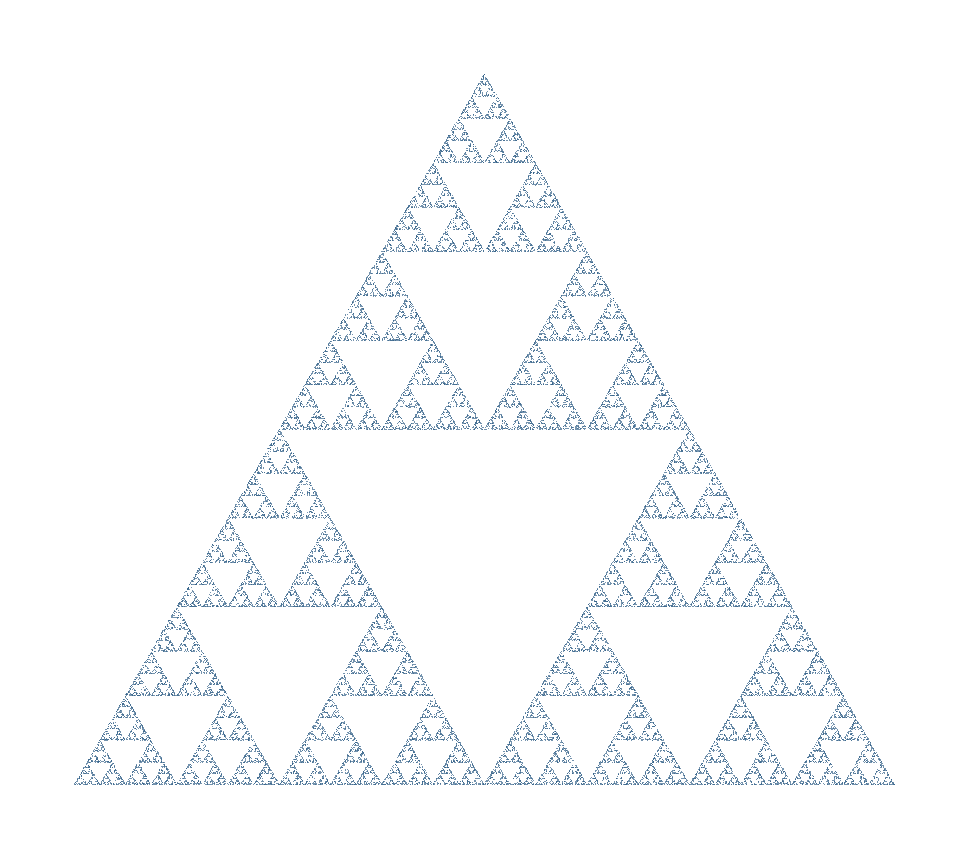
\includegraphics{py-sierpinski.png}}
    \end{column}
    \begin{column}{0.55\textwidth}
      \small
      Partant d'un point, on choisit au hasard, à répétition, l'un des
      trois sommets d'un triangle, et on avance à mi-chemin
      vers lui.
      \vspace{6pt}

      Pourquoi obtient-on toujours la même figure ?
      \begin{itemize}
        \item Réponse au chapitre 3, grâce au théorème du point
          fixe de Banach --- démontré aujourd'hui.
        \item La figure sera un point d'un espace dont les
          « points » sont des ensembles compacts du plan, muni de la
          distance de Hausdorff --- construite aujourd'hui.
      \end{itemize}
    \end{column}
  \end{columns}
\end{frame}

\begin{frame}{Le chemin de ce chapitre}
  \FigBox[0.42\textheight]{%
    \begin{tikzpicture}[
        etape/.style={draw=sectioncolor, fill=thmboxbg, rounded corners=2pt,
          thick, align=center, font=\scriptsize, minimum height=1.05cm,
          text width=2.05cm},
        but/.style={etape, draw=coveraccent!85!black, fill=secboxbg}]
      \node[etape] (m) at (0,0) {Métrique\\$(E,d)$};
      \node[etape] (o) at (2.6,0) {Ouverts, fermés,\\compacts};
      \node[etape] (h) at (5.2,0) {Distance de\\Hausdorff $\dH$};
      \node[etape] (c) at (2.6,-1.7) {Suites de Cauchy,\\complétude};
      \node[etape] (k) at (5.2,-1.7) {Points fixes,\\contractions};
      \node[but] (b) at (8.1,-0.85) {Théorème\\de Banach};
      \node[etape, text width=2.3cm] (n) at (11.0,0) {Méthode de\\Newton};
      \node[etape, text width=2.3cm] (f) at (11.0,-1.7) {Fractales\\(chapitre 3)};
      \draw[fleche] (m) -- (o);
      \draw[fleche] (o) -- (h);
      \draw[fleche] (m) |- (c);
      \draw[fleche] (c) -- (k);
      \draw[fleche] (k) -- (b);
      \draw[fleche] (h) -- (b);
      \draw[fleche] (b) -- (n);
      \draw[fleche] (b) -- (f);
    \end{tikzpicture}}
  \small Deux applications tout au long du chemin : la
  navigation sur une sphère et la détection d'erreurs
  dans une chaîne de bits.
\end{frame}

% ═══════════════════════════════════════════════════════════════════════
\section{Qu'est-ce qu'une distance ?}
% ═══════════════════════════════════════════════════════════════════════

\begin{frame}{Ce que l'on sait déjà de la distance euclidienne}
  Si $P$, $Q$, $R$ sont trois points du plan :
  \begin{enumerate}
    \item $d(P,Q)$ est toujours un nombre positif ou nul ;
    \item $d(P,Q) = 0$ exactement quand $P$ et $Q$ sont le même point ;
    \item $d(P,Q) = d(Q,P)$ ;
    \item $d(P,Q) \leq d(P,R) + d(R,Q)$ : un détour par $R$ n'est jamais
      plus court que le chemin direct.
  \end{enumerate}
  \vspace{6pt}
  \begin{Rem}{Observation}
    Ces quatre propriétés ne font intervenir ni les
    coordonnées, ni le fait que $P,Q,R$ soient des points du plan. On
    peut donc les reprendre telles quelles sur un ensemble quelconque.
  \end{Rem}
\end{frame}

\begin{frame}{Définition 2.1 --- Métrique, espace métrique}
  \begin{Enonce}{Définition 2.1 --- Métrique, espace métrique}
    Soit $E$ un ensemble. Une \defi{métrique} (ou \defi{distance}) sur
    $E$ est une fonction $d : E\times E\to\R$ telle que, pour tous
    $x,y,z\in E$ :
    \begin{center}
    \begin{tabular}{lll}
      (a) & $d(x,y)\geq 0$ & (positivité) \\
      (b) & $d(x,y)=0 \iff x=y$ & (séparation) \\
      (c) & $d(x,y)=d(y,x)$ & (symétrie) \\
      (d) & $d(x,y)\leq d(x,z)+d(z,y)$ & (inégalité triangulaire)
    \end{tabular}
    \end{center}
    Le couple $(E,d)$ s'appelle alors un \defi{espace métrique}.
  \end{Enonce}
\end{frame}

\begin{frame}{Figure 2.2 --- L'inégalité triangulaire}
  \FigBox[0.45\textheight]{%
    \begin{tikzpicture}[scale=1.25]
      \node[pt, label={[etiq]below:$x$}] (x) at (0,0) {};
      \node[pt, label={[etiq]right:$y$}] (y) at (3.4,0.5) {};
      \node[pt, label={[etiq]above:$z$}] (z) at (1.3,2.1) {};
      \draw[sectioncolor, thick] (x) -- (y) node[midway, below, etiq]{$d(x,y)$};
      \draw[sectioncolor!70, thick, dashed] (x) -- (z) node[midway, left, etiq]{$d(x,z)$};
      \draw[sectioncolor!70, thick, dashed] (z) -- (y) node[midway, above right, etiq]{$d(z,y)$};
    \end{tikzpicture}}
  \small Le nom vient du cas $E=\R^2$ : dans un triangle, chaque côté est
  au plus égal à la somme des deux autres. La propriété du secondaire
  devient un axiome, valable pour des ensembles beaucoup plus
  généraux.
\end{frame}

\begin{frame}{Remarque 2.1 --- La propriété de séparation}
  \begin{Rem}{Remarque 2.1}
    La condition (b) réunit deux implications à distinguer :
    \begin{itemize}
      \item $d(x,x)=0$ pour tout $x$ : la distance d'un point à
        lui-même est nulle (intuitif) ;
      \item si $d(x,y)=0$, alors $x=y$ : seuls deux points
        confondus sont à distance nulle.
    \end{itemize}
    D'où le nom : une métrique sépare toujours deux points
    distincts par une distance strictement positive.
  \end{Rem}
  \vspace{6pt}
  \small Cette condition devra être vérifiée avec attention pour la
  distance de Hausdorff (section 5).
\end{frame}

\subsection{Les distances euclidienne et de Manhattan}

\begin{frame}{Exemple 2.1 --- La distance euclidienne dans $\R$ et $\R^n$}
  \small
  Sur $\R$ : $\dE(x,y) = |x-y|$. Positivité, séparation, symétrie :
  propriétés de la valeur absolue. Inégalité triangulaire :
  $|a+b|\leq|a|+|b|$ avec $a=x-z$, $b=z-y$.

  \vspace{6pt}
  Sur $\R^n$, pour $X=(x_1,\dots,x_n)$ et $Y=(y_1,\dots,y_n)$ :
  \[
    \dE(X,Y) = \sqrt{\sum_{i=1}^{n}(x_i-y_i)^2}\,,
  \]
  la distance euclidienne. Pour $n=2$ : le théorème de Pythagore
  appliqué à la différence des coordonnées.

  \vspace{6pt}
  Convention : sauf mention contraire, c'est la métrique
  utilisée sur $\R^n$.
\end{frame}

\begin{frame}{Exemple 2.2 --- La taxi-distance}
  \begin{columns}[c]
    \begin{column}{0.48\textwidth}
      \small Pour $X=(x_1,y_1)$, $Y=(x_2,y_2)$ dans $\R^2$ :
      \[
        \dT(X,Y) = |x_2-x_1| + |y_2-y_1|.
      \]
      Une autre métrique sur $\R^2$ (inégalité triangulaire : coordonnée
      par coordonnée). C'est la taxi-distance, ou distance
      de Manhattan : un taxi sur un quadrillage de rues
      perpendiculaires, sans trajet diagonal.
    \end{column}
    \begin{column}{0.5\textwidth}
      \FigBox[0.6\textheight]{%
        \begin{tikzpicture}[scale=0.62]
          \draw[quadrillage] (-0.4,-0.4) grid (7.4,5.4);
          \node[pt, label={[etiq]below left:$A$}] (A) at (1,1) {};
          \node[pt, label={[etiq]above right:$B$}] (B) at (6,4) {};
          \draw[sectioncolor, thick] (A) -- (B);
          \node[etiq, sectioncolor] at (3.5,5.0) {$\dE(A,B) = \sqrt{5^2+3^2}=\sqrt{34}$};
          \draw[firebrick3, very thick]
            (1,1) -- (2,1) -- (2,2) -- (3,2) -- (3,3) -- (4,3) -- (5,3) -- (5,4) -- (6,4);
          \node[etiq, firebrick3] at (3.5,0.5) {$\dT(A,B) = 5 + 3 = 8$};
        \end{tikzpicture}}
      \begin{center}\scriptsize Figure 2.3 --- Tout chemin en escalier a
      la même longueur.\end{center}
    \end{column}
  \end{columns}
\end{frame}

\begin{frame}{Remarque 2.2 --- Même paire de points, deux distances}
  \begin{Rem}{Remarque 2.2}
    $\dE$ et $\dT$ sont deux métriques distinctes sur le
    même ensemble $\R^2$ : sur la figure 2.3,
    $\sqrt{34}\approx\num{5.83}$ contre $8$.
    \vspace{4pt}

    Un même ensemble, deux métriques : deux espaces métriques
    différents, $(\R^2,\dE)$ et $(\R^2,\dT)$, bien qu'ils aient
    les mêmes éléments.
  \end{Rem}
  \vspace{6pt}
  \small À retenir pour la section 4 : la forme d'une boule
  dépend de la métrique, pas seulement de l'ensemble.
\end{frame}

% ═══════════════════════════════════════════════════════════════════════
\section{Deux métriques appliquées : la sphère et les bits}
% ═══════════════════════════════════════════════════════════════════════

\subsection{La distance sur la sphère}

\begin{frame}{La distance sphérique}
  \begin{columns}[c]
    \begin{column}{0.52\textwidth}
      \small
      \begin{itemize}
        \item Le segment Montréal--Paris passe à l'intérieur de
          la Terre : un avion ne peut pas le suivre.
        \item On mesure plutôt le long de l'arc de grand cercle :
          l'intersection de la sphère avec le plan passant par $u$, $v$
          et le centre $O$.
        \item Cette longueur d'arc est la distance sphérique (ou
          du grand cercle) : le plus court chemin le long de la
          surface.
      \end{itemize}
      \vspace{2pt}
      \scriptsize Navigation aérienne, GPS : c'est pourquoi les vols vers
      l'Europe semblent « courber vers le nord » sur une carte plane.
    \end{column}
    \begin{column}{0.46\textwidth}
      \FigBox[0.62\textheight]{%
        \begin{tikzpicture}[scale=1.3]
          \draw[sectioncolor, thick] (0,0) circle (2);
          \draw[sectioncolor!45, thick] (0,0) ellipse (2 and 0.55);
          \draw[sectioncolor!25, thick, dashed] (-2,0) arc (180:360:2 and 0.55);
          \node[pt, label={[etiq]above left:$u$}] (u) at (-1.05,1.1) {};
          \node[pt, label={[etiq]above right:$v$}] (v) at (1.35,0.75) {};
          \node[etiq] at (0,-0.22) {$O$};
          \fill (0,0) circle (0.6pt);
          \draw[firebrick3, thick, dashed] (u) -- (v);
          \node[etiq, firebrick3] at (0.5,0.65) {corde};
          \draw[sectioncolor, very thick] (u) to[bend left=35] (v);
          \node[etiq, sectioncolor] at (0.15,1.55) {arc};
          \draw[sectioncolor!60, thin] (0,0) -- (u);
          \draw[sectioncolor!60, thin] (0,0) -- (v);
        \end{tikzpicture}}
      \begin{center}\scriptsize Figure 2.4\end{center}
    \end{column}
  \end{columns}
\end{frame}

\subsection{Mesurer les erreurs}

\begin{frame}{Définition 2.2 --- Distance de Hamming}
  \small Un message binaire transmis peut voir certains bits inversés par
  le bruit (canal informatique, disque, satellite). Pour détecter ---
  voire corriger --- ces erreurs, il faut d'abord mesurer l'écart
  entre deux messages.
  \begin{Enonce}{Définition 2.2 --- Distance de Hamming}
    Soit $n\in\Ns$. Pour $X=(x_1,\dots,x_n)$ et $Y=(y_1,\dots,y_n)$
    dans $\{0,1\}^n$,
    \[
      \dHam(X,Y) = \sum_{i=1}^{n}|x_i-y_i|.
    \]
  \end{Enonce}
  \small Comme $|x_i-y_i|\in\{0,1\}$, $\dHam(X,Y)$ est le nombre
  de positions où $X$ et $Y$ diffèrent : le nombre minimal de bits à
  inverser pour passer de $X$ à $Y$.
\end{frame}

\begin{frame}{Exemple 2.3 --- Un calcul de distance de Hamming}
  \small $X=(1,0,0,1)$ et $Y=(1,1,0,0)$ dans $\{0,1\}^4$ :
  \[
    \dHam(X,Y) = |1-1|+|0-1|+|0-0|+|1-0| = 0+1+0+1 = 2.
  \]
  \FigBox[0.32\textheight]{%
    \begin{tikzpicture}[scale=1, every node/.style={font=\sffamily}]
      \foreach \i/\xb/\yb/\same in {1/1/1/1, 2/0/1/0, 3/0/0/1, 4/1/0/0} {
        \pgfmathsetmacro{\xoff}{(\i-1)*1.05}
        \node[draw=sectioncolor, thick, fill=steelblue4!15, minimum size=0.85cm]
          at (\xoff,0.55) {\xb};
        \ifnum\same=1
          \node[draw=sectioncolor, thick, fill=steelblue4!15, minimum size=0.85cm]
            at (\xoff,-0.55) {\yb};
        \else
          \node[draw=firebrick3, thick, fill=firebrick3!20, minimum size=0.85cm]
            at (\xoff,-0.55) {\yb};
        \fi
      }
      \node[etiq, left] at (-0.7,0.55) {$X$};
      \node[etiq, left] at (-0.7,-0.55) {$Y$};
    \end{tikzpicture}}
  \small Les suites diffèrent exactement aux positions 2 et 4.
\end{frame}

\begin{frame}{$\dHam$ est bien une métrique}
  \small
  \begin{itemize}
    \item Somme de valeurs absolues : positive ou nulle ; nulle
      exactement quand chaque terme l'est, i.e. $X=Y$.
    \item $|x_i-y_i| = |y_i-x_i|$ : symétrie.
  \end{itemize}
  \begin{AuTableau}[Vérification au tableau]
    \small Inégalité triangulaire, position par position : si $X$ et $Y$
    diffèrent en $i$ mais pas $X$ et $Z$, alors $Z$ et $Y$ y diffèrent
    forcément. Chaque position comptée à gauche dans
    $\dHam(X,Y)\leq\dHam(X,Z)+\dHam(Z,Y)$ l'est au moins une fois à
    droite.
  \end{AuTableau}
\end{frame}

\begin{frame}{Note historique 2.1 --- Richard Hamming et la détection d'erreurs}
  \small
  \begin{itemize}
    \item 1950, laboratoires Bell : Richard Hamming (1915--1998)
      travaille sur la fiabilité des premiers ordinateurs à relais.
    \item Les arrêts de la machine les fins de semaine l'irritent : elle
      détecte une erreur de lecture, mais ne sait pas la
      corriger.
    \item Son idée --- les codes de Hamming : choisir les messages
      valides tous à distance de Hamming au moins 3 les uns des
      autres.
    \item Un message corrompu par une erreur reste alors
      strictement plus proche (au sens de $\dHam$) du message original
      que de tout autre message valide : on le corrige automatiquement.
  \end{itemize}
  \vspace{4pt}
  Même idée aujourd'hui, sous une forme ou une autre, dans les CD, les
  disques durs, les communications par satellite.
\end{frame}

% ═══════════════════════════════════════════════════════════════════════
\section{Ouverts, fermés et compacts}
% ═══════════════════════════════════════════════════════════════════════

\begin{frame}{Pourquoi ce détour ?}
  \small Avant de définir une distance entre deux ensembles, il
  faut le vocabulaire des ensembles ouverts, fermés et
  compacts.
  \begin{itemize}
    \item Tout repose sur une seule notion : la boule ouverte.
    \item Tout s'exprime dans le langage des espaces métriques.
    \item On illustre surtout dans $\R^n$, où l'interprétation
      géométrique est la plus parlante.
  \end{itemize}
\end{frame}

\subsection{Boules et ensembles ouverts}

\begin{frame}{Définition 2.3 --- Boule ouverte}
  \begin{Enonce}{Définition 2.3 --- Boule ouverte}
    Soit $(E,d)$ un espace métrique, $x_0\in E$ et $r>0$. La \defi{boule
    ouverte} de centre $x_0$ et de rayon $r$ est
    \[
      \boule{x_0}{r} = \{x\in E : d(x,x_0) < r\}.
    \]
  \end{Enonce}
  \FigBox[0.4\textheight]{%
    \begin{tikzpicture}[scale=0.85]
      \begin{scope}
        \draw[sectioncolor, thick, dashed, fill=steelblue4!15] (0,0) circle (1.4);
        \node[pt] (c) at (0,0) {};
        \node[etiq, below] at (0,0) {$x_0$};
        \draw[sectioncolor!70, thick, dashed] (0,0) -- (45:1.4) node[midway, above, etiq]{$r$};
        \node[etiq, sectioncolor] at (0,-1.9) {$\boule{x_0}{r}$ dans $(\R^2,\dE)$};
      \end{scope}
      \begin{scope}[xshift=5.4cm]
        \draw[firebrick3, thick, dashed, fill=firebrick3!15]
          (0,1.4) -- (1.4,0) -- (0,-1.4) -- (-1.4,0) -- cycle;
        \node[pt] (c2) at (0,0) {};
        \node[etiq, below] at (0,0) {$x_0$};
        \draw[firebrick3!70, thick, dashed] (0,0) -- (0.7,0.7) node[midway, above, etiq]{$r$};
        \node[etiq, firebrick3] at (0,-1.9) {$\boule{x_0}{r}$ dans $(\R^2,\dT)$};
      \end{scope}
    \end{tikzpicture}}
  \begin{center}\scriptsize Figure 2.5 --- Même ensemble, même centre :
  un disque pour $\dE$, un carré tourné de $45^\circ$ pour $\dT$
  ($|x-x_0|+|y-y_0|<r$).\end{center}
\end{frame}

\begin{frame}{Outil 2.1 --- Tracer des boules dans Desmos}
  \begin{Outil}{Tracer des boules dans Desmos}
    \small Desmos trace directement les régions définies par des
    inégalités :
    \begin{center}
      \texttt{x\^{}2 + y\^{}2 < r\^{}2} \qquad et \qquad
      \texttt{|x| + |y| < r},
    \end{center}
    avec un curseur pour $r$ : on obtient les deux boules de la
    figure 2.5. Le bord est tracé en pointillé --- il
    n'appartient pas à la boule ouverte. Avec \texttt{<=}, le bord
    devient plein : boule ouverte vs boule fermée, visuellement.
    \vspace{4pt}

    En $4^{\text{e}}$ secondaire : comparer « à vol d'oiseau » et « en
    taxi » à partir d'un point donné.
  \end{Outil}
\end{frame}

\begin{frame}{Définition 2.4 --- Ensemble ouvert}
  \begin{Enonce}{Définition 2.4 --- Ensemble ouvert}
    Soit $(E,d)$ un espace métrique et $U\subseteq E$. $U$ est un
    \defi{ensemble ouvert} si, pour tout $x\in U$, il existe $r>0$ tel
    que $\boule{x}{r}\subseteq U$.
  \end{Enonce}
  \small Chaque point de $U$ est le centre d'une boule entièrement
  contenue dans $U$ : aucun point de $U$ n'est sur sa frontière. Le
  rayon peut dépendre du point --- plus petit près du bord, mais
  toujours strictement positif.
\end{frame}

\begin{frame}{Figures 2.6 et 2.7 --- Ouvert, et pas ouvert}
  \begin{columns}[T]
    \begin{column}{0.5\textwidth}
      \FigBox[0.42\textheight]{%
        \begin{tikzpicture}[scale=0.85]
          \draw[fig, dashed] plot[smooth cycle, tension=0.8]
            coordinates {(0,0) (1.3,-0.7) (2.8,-0.3) (3.2,1.1) (2.1,2.2) (0.7,1.9) (-0.5,1)};
          \node[pt, label={[etiq]above:$x_1$}] (x1) at (1.4,0.6) {};
          \draw[sectioncolor!60, thick, dashed] (x1) circle (0.55);
          \node[pt, label={[etiq]below:$x_2$}] (x2) at (2.5,1.6) {};
          \draw[sectioncolor!60, thick, dashed] (x2) circle (0.22);
        \end{tikzpicture}}
      \scriptsize Figure 2.6. Un ouvert (frontière en pointillé,
      exclue). Près du bord, $x_2$ demande un rayon plus petit que $x_1$
      --- mais il en existe un.
    \end{column}
    \begin{column}{0.46\textwidth}
      \FigBox[0.42\textheight]{%
        \begin{tikzpicture}[scale=0.85]
          \draw[fig] (0,0) circle (1.4);
          \node[pt, label={[etiq]right:$x_2$}] (x2b) at (1.4,0) {};
          \draw[firebrick3, thick, dashed] (x2b) circle (0.4);
        \end{tikzpicture}}
      \scriptsize Figure 2.7. Le disque plein, bord compris,
      n'est pas ouvert : toute boule centrée en $x_2$, même
      minuscule, déborde du disque.
    \end{column}
  \end{columns}
\end{frame}

\subsection{Ensembles fermés}

\begin{frame}{Définition 2.5 --- Ensemble fermé}
  \begin{Enonce}{Définition 2.5 --- Ensemble fermé}
    Soit $(E,d)$ un espace métrique et $F\subseteq E$. $F$ est un
    \defi{ensemble fermé} si son complément $\comp{F}$ est ouvert dans
    $(E,d)$.
  \end{Enonce}
  \vspace{4pt}
  \begin{Rem}{Remarque 2.3 --- Ni l'un ni l'autre, ou les deux}
    « Ouvert » et « fermé » ne s'excluent pas :
    \begin{itemize}
      \item un ensemble peut n'être ni l'un ni l'autre (un disque qui
        contient une partie, mais pas la totalité, de sa frontière) ;
      \item $E$ et $\emptyset$ sont à la fois ouverts et fermés
        dans $(E,d)$.
    \end{itemize}
  \end{Rem}
\end{frame}

\subsection{Ensembles compacts}

\begin{frame}{Définition 2.6 et théorème 2.1 --- Borné, compact}
  \begin{Enonce}{Définition 2.6 --- Ensemble borné}
    Soit $(E,d)$ un espace métrique et $F\subseteq E$. $F$ est
    \defi{borné} s'il existe $c\in\R$ tel que $d(x,y)\leq c$ pour tous
    $x,y\in F$.
  \end{Enonce}
  \begin{Enonce}{Théorème 2.1 --- Heine-Borel}
    Soit $K\subseteq\R^n$, muni de $\dE$. $K$ est compact si et
    seulement s'il est à la fois fermé et borné.
  \end{Enonce}
  \small (Admis.) Convention du chapitre : dans $\R^n$, on
  utilise « fermé et borné » comme définition d'un compact.
\end{frame}

\begin{frame}{Remarque 2.4 --- La compacité dans un espace général}
  \begin{Rem}{Remarque 2.4}
    « Fermé et borné » n'est pas, à proprement parler, la
    définition d'un compact : c'en est une
    caractérisation, valable dans $\R^n$, qui cesse d'être
    vraie dans des espaces métriques plus généraux.
    \vspace{4pt}

    La véritable définition : de tout recouvrement de $K$ par des
    ouverts, on peut extraire un nombre fini d'ouverts qui
    recouvrent encore $K$.
  \end{Rem}
  \vspace{4pt}
  \small Pour nos besoins --- dans $\R^n$ --- « fermé et borné »
  suffira.
\end{frame}

% ═══════════════════════════════════════════════════════════════════════
\section{La distance de Hausdorff}
% ═══════════════════════════════════════════════════════════════════════

\begin{frame}{Une distance entre des ensembles}
  \small Notons $\Comp{E}$ l'ensemble des sous-ensembles compacts
  non vides d'un espace métrique $(E,d)$.
  \vspace{6pt}

  L'idée à formaliser : deux ensembles sont proches lorsque
  chaque point de l'un est près d'un point de l'autre, et
  réciproquement.
  \vspace{6pt}

  Outil : le voisinage d'un ensemble, obtenu en l'« épaississant ».
  \vspace{6pt}

  Objectif lointain : au chapitre 3, une figure fractale sera
  un point de l'espace métrique $\big(\Comp{\R^2},\dH\big)$.
\end{frame}

\subsection[Le epsilon-voisinage et la somme de Minkowski]{Le \texorpdfstring{$\varepsilon$}{epsilon}-voisinage et la somme de Minkowski}

\begin{frame}{Définitions 2.7 et 2.8 --- Minkowski, $\varepsilon$-voisinage}
  \begin{Enonce}{Définition 2.7 --- Somme de Minkowski}
    \small Soit $(E,d)=(\R^n,\dE)$ et $A,B\subseteq E$. La \defi{somme de
    Minkowski} de $A$ et $B$ est
    $A\oplus B = \{a+b : a\in A,\ b\in B\}$.
  \end{Enonce}
  \small Une copie de $B$ placée en chaque point de $A$, puis on réunit
  tout. Si $B$ est une petite boule fermée centrée à l'origine : on
  ajoute autour de $A$ une bande de même épaisseur dans toutes les
  directions.
  \begin{Enonce}{Définition 2.8 --- $\varepsilon$-voisinage d'un ensemble}
    \small Soit $A\subseteq\R^n$ non vide et $\varepsilon>0$. Le
    \defi{$\varepsilon$-voisinage} de $A$ est
    $\Vois{A}{\varepsilon} = A\oplus\overline{\boule{0}{\varepsilon}}$,
    où $\overline{\boule{0}{\varepsilon}} = \{x : \dE(x,0)\leq\varepsilon\}$
    est la boule fermée.
  \end{Enonce}
\end{frame}

\begin{frame}{Figure 2.8 --- Le $\varepsilon$-voisinage}
  \begin{columns}[c]
    \begin{column}{0.5\textwidth}
      \small Reformulation :
      \[
        \begin{aligned}
          \Vois{A}{\varepsilon} = \{x\in E :\ & \dE(x,a)\leq\varepsilon\\
          & \text{pour un certain } a\in A\},
        \end{aligned}
      \]
      les points à distance au plus $\varepsilon$ d'au moins un
      point de $A$.
      \vspace{6pt}

      En particulier $A\subseteq\Vois{A}{\varepsilon}$ : chaque point
      de $A$ est à distance $0\leq\varepsilon$ de lui-même.
    \end{column}
    \begin{column}{0.48\textwidth}
      \FigBox[0.55\textheight]{%
        \begin{tikzpicture}[scale=0.9]
          \draw[sectioncolor, thick, fill=steelblue4!28] plot[smooth cycle, tension=0.75]
            coordinates {(-0.49,-0.20) (0.99,-1.01) (2.75,-0.47) (3.16,1.02)
                         (1.81,2.23) (0.19,1.83)};
          \draw[fig] plot[smooth cycle, tension=0.75]
            coordinates {(0,0) (1.1,-0.6) (2.4,-0.2) (2.7,0.9) (1.7,1.8) (0.5,1.5)};
          \node[etiq, sectioncolor] at (1.2,0.6) {$A$};
          \node[etiq, sectioncolor] at (2.7,2.35) {$\Vois{A}{\varepsilon}$};
          \draw[fleche, sectioncolor] (1.85,1.55) -- (2.5,2.05);
          \draw[sectioncolor, thick, {Stealth[length=2mm]}-{Stealth[length=2mm]}]
            (2.1,-0.3) -- (2.8,-0.3);
          \node[etiq, sectioncolor, below] at (2.45,-0.35) {$\varepsilon$};
        \end{tikzpicture}}
      \scriptsize (Dessin simplifié : une homothétie plutôt que la vraie
      somme de Minkowski.)
    \end{column}
  \end{columns}
\end{frame}

\begin{frame}{Remarque 2.5 --- Le voisinage dépend aussi de la métrique}
  \begin{Rem}{Remarque 2.5}
    Comme les boules (figure 2.5), le $\varepsilon$-voisinage change
    d'aspect avec la métrique. Pour le singleton $A=\{(0,0)\}$ :
    \begin{itemize}
      \item avec une boule fermée de $(\R^2,\dE)$ : un disque
        plein de rayon $\varepsilon$ ;
      \item avec une boule fermée de $(\R^2,\dT)$ : un carré
        plein tourné de $45^\circ$, de « demi-diagonale » $\varepsilon$.
    \end{itemize}
  \end{Rem}
\end{frame}

\subsection{Définition de la distance de Hausdorff}

\begin{frame}{Définition 2.9 --- Distance de Hausdorff}
  \begin{Enonce}{Définition 2.9 --- Distance de Hausdorff}
    Soit $(E,d)=(\R^n,\dE)$ et $A,B\in\Comp{E}$. La \defi{distance de
    Hausdorff} entre $A$ et $B$ est
    \[
      \dH(A,B) = \inf\{\varepsilon>0 : A\subseteq\Vois{B}{\varepsilon}
      \text{ et } B\subseteq\Vois{A}{\varepsilon}\}.
    \]
  \end{Enonce}
  \small Le plus petit rayon d'épaississement tel que chacun des
  deux ensembles soit recouvert par le $\varepsilon$-voisinage de
  l'autre.
  \begin{itemize}
    \item $A$, $B$ compacts donc bornés : un tel $\varepsilon$ existe
      toujours (assez grand).
    \item On peut montrer que l'infimum est en fait atteint.
  \end{itemize}
\end{frame}

\begin{frame}{Figure 2.9 --- La formule de calcul}
  \begin{columns}[c]
    \begin{column}{0.5\textwidth}
      \small Avec $d(x,C) = \inf_{c\in C} d(x,c)$ :
      \[
        \dH(A,B) = \max\Big\{\sup_{a\in A} d(a,B),\ \sup_{b\in B} d(b,A)\Big\}.
        \tag{2.1}
      \]
      Recette : trouver le point de $A$ le plus loin de $B$ ;
      puis le point de $B$ le plus loin de $A$ ; garder la plus grande
      des deux distances.
    \end{column}
    \begin{column}{0.48\textwidth}
      \FigBox[0.55\textheight]{%
        \begin{tikzpicture}[scale=1.15]
          \draw[firebrick3, thick, fill=firebrick3, fill opacity=0.3] (0,0) circle (1.3);
          \node[etiq, firebrick3] at (-0.75,0.95) {$B$};
          \draw[sectioncolor, thick, fill=steelblue4, fill opacity=0.3,
                rotate around={10:(1.8,0.2)}] (1.8,0.2) ellipse (1.6 and 0.85);
          \node[etiq, sectioncolor] at (2.55,1.15) {$A$};
          \node[pt, label={[etiq]above right:$a^\star$}] (astar) at (3.38,0.48) {};
          \node[ptim, label={[etiq]left:$b^\star$}] (bstar) at (-1.3,0) {};
          \draw[sectioncolor!70, thick, dashed, {Stealth[length=2mm]}-{Stealth[length=2mm]}]
            (astar) -- node[midway, below, etiq]{$d(a^\star,B)$} (1.29,0.18);
          \draw[firebrick3!70, thick, dashed, {Stealth[length=2mm]}-{Stealth[length=2mm]}]
            (bstar) -- node[midway, above, etiq]{$d(b^\star,A)$} (0.22,-0.08);
        \end{tikzpicture}}
    \end{column}
  \end{columns}
\end{frame}

\begin{frame}{Exemple 2.4 --- Deux carrés emboîtés}
  \begin{columns}[c]
    \begin{column}{0.58\textwidth}
      \small $A=\intff{0}{2}\times\intff{0}{2}$,
      $B=\intff{0}{3}\times\intff{0}{3}$.
      \begin{itemize}
        \item $A\subseteq B$ : tout point de $A$ est à distance $0$ de
          $B$, donc $\sup_{a\in A}d(a,B)=0$.
        \item Le point de $B$ le plus loin de $A$ : le coin $(3,3)$, à
          distance $\dE\big((3,3),(2,2)\big)=\sqrt2$.
      \end{itemize}
      \[
        \dH(A,B) = \max\{0,\sqrt2\} = \sqrt2.
      \]
      \scriptsize La formule (2.1) n'est pas symétrique terme à
      terme : c'est le $\max$ qui rend $\dH$ symétrique.
    \end{column}
    \begin{column}{0.4\textwidth}
      \FigBox[0.55\textheight]{%
        \begin{tikzpicture}[scale=0.9]
          \repere{-0.4}{3.4}{-0.4}{3.4}
          \fill[figim] (0,0) rectangle (3,3);
          \fill[fig] (0,0) rectangle (2,2);
          \node[etiq, sectioncolor] at (1,1) {$A$};
          \node[etiq, firebrick3] at (2.6,0.6) {$B$};
          \node[ptim, label={[etiq]above right:$(3,3)$}] (p) at (3,3) {};
          \node[pt] (q) at (2,2) {};
          \draw[firebrick3, thick, dashed] (q) -- node[etiq, above left]{$\sqrt2$} (p);
        \end{tikzpicture}}
    \end{column}
  \end{columns}
\end{frame}

\begin{frame}{Remarque 2.6 --- Pourquoi des ensembles compacts ?}
  \begin{Rem}{Remarque 2.6}
    \small La restriction aux compacts sert à garantir la
    séparation (axiome (b)).
    \vspace{4pt}

    Contre-exemple sans compacité : dans $(\R,\dE)$,
    $A=\intoo{0}{1}$ et $B=\intff{0}{1}$ sont distincts, et pourtant
    $\dH(A,B)=0$ : tout point de $B$ est aussi près qu'on veut d'un
    point de $A$. Le coupable : $A$ n'est pas fermé, il lui « manque »
    ses points frontières.
    \vspace{4pt}

    Sur $\Comp{E}$, on démontre que $\dH(A,B)=0 \Rightarrow A=B$ ; on
    vérifie aussi symétrie et inégalité triangulaire.
  \end{Rem}
  \vspace{4pt}
  \begin{center}
    $(\Comp{E},\dH)$ est un espace métrique dont les « points »
    sont des ensembles.
  \end{center}
\end{frame}

\begin{frame}{Pour la classe 2.1 --- Comparer deux figures géométriques}
  \begin{Classe}{Comparer deux figures géométriques}
    \small « À quel point ce triangle ressemble-t-il à celui-là ? » La
    distance de Hausdorff rend la question précise :
    \begin{itemize}
      \item deux polygones de forme presque identique, dont un sommet a
        légèrement bougé : petite distance de Hausdorff ;
      \item des figures plus différentes : distance plus grande.
    \end{itemize}
    \vspace{2pt}
    C'est le principe de certains logiciels de reconnaissance de
    formes : un contour détecté dans une image ressemble-t-il
    suffisamment à un contour de référence ?
  \end{Classe}
\end{frame}

\begin{frame}{Note historique 2.2 --- Felix Hausdorff (1868--1942)}
  \footnotesize
  \begin{columns}[T]
    \begin{column}{0.25\textwidth}
      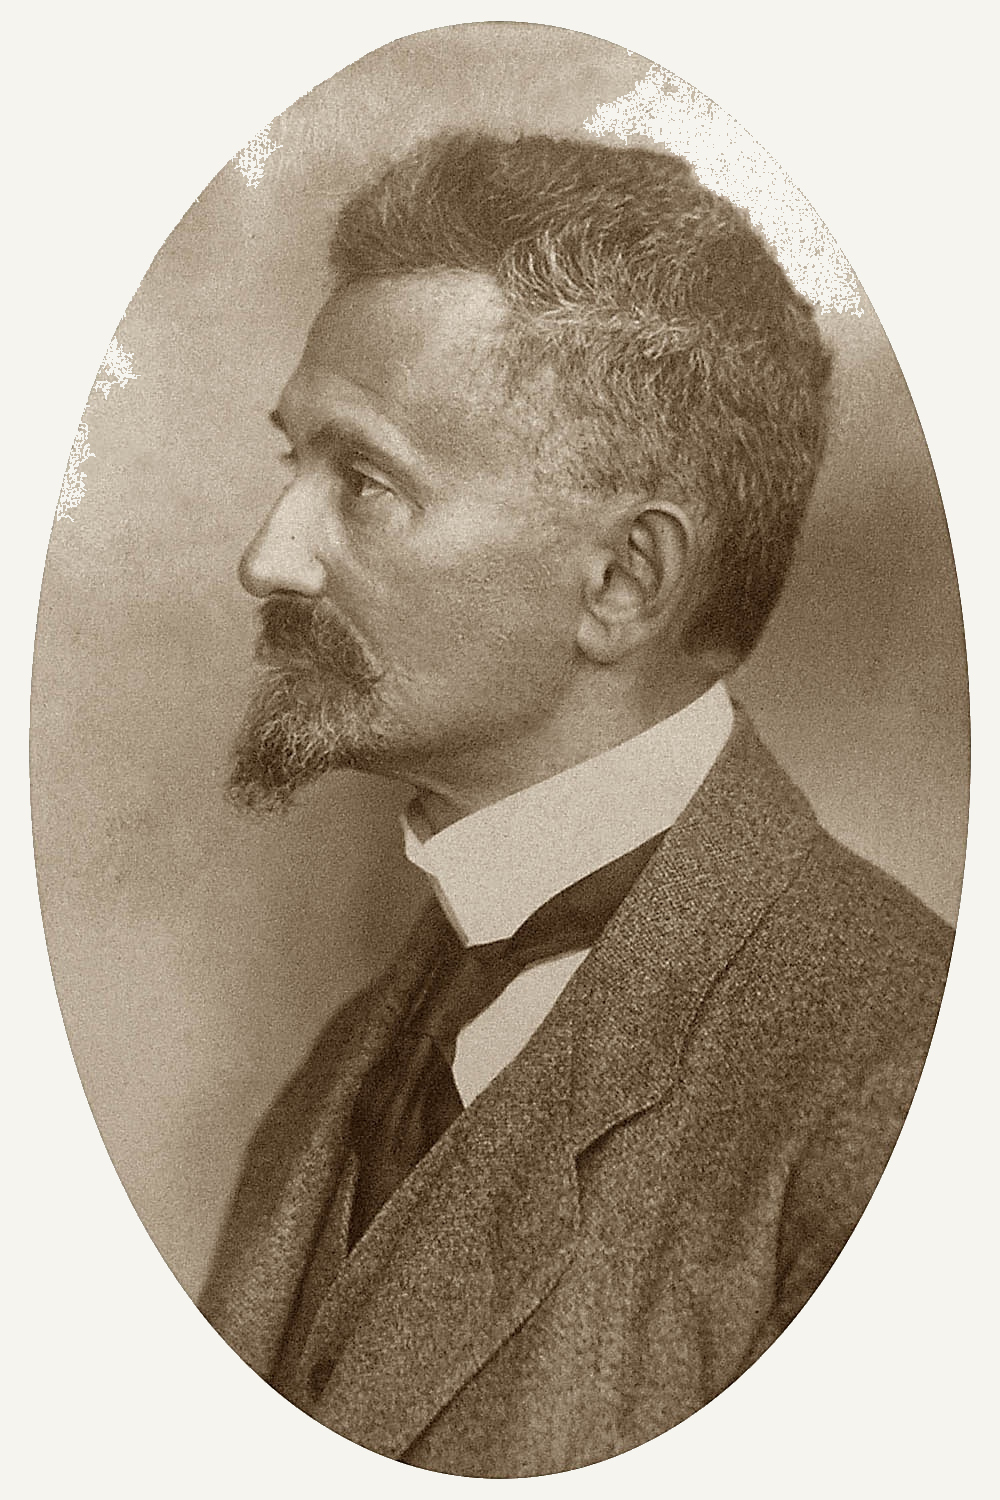
\includegraphics[width=\linewidth]{felix-hausdorff.jpg}\\
      {\scriptsize\color{gray}Felix Hausdorff (1868--1942).
      Domaine public, Wikimedia Commons.}
    \end{column}
    \begin{column}{0.72\textwidth}
      \begin{itemize}
        \item Mathématicien allemand, professeur à Leipzig, Bonn et
          Greifswald.
        \item Grundzüge der Mengenlehre (1914) : les bases de la
          topologie générale telle qu'on l'enseigne encore ;
          c'est là qu'apparaît la distance qui porte son nom.
        \item Aussi poète, essayiste (sur Nietzsche) et dramaturge, sous
          le pseudonyme Paul Mongré.
      \end{itemize}
    \end{column}
  \end{columns}
\end{frame}

\begin{frame}{Note historique 2.2 (suite)}
  \small
  \begin{itemize}
    \item À partir de 1933, persécuté par le régime nazi en raison de
      ses origines juives ; mis à la retraite forcée en 1935 « sans un
      mot de remerciement ».
    \item Après la Nuit de Cristal (1938), ses conditions se
      détériorent encore ; une tentative d'émigration vers les
      États-Unis échoue en 1939.
    \item En janvier 1942, recevant l'ordre de se présenter à un camp
      d'internement, il se donne la mort avec son épouse Charlotte et
      la sœur de celle-ci. Il avait 73 ans.
  \end{itemize}
  \vspace{4pt}
  Une partie de son œuvre, dont la dimension de Hausdorff ---
  outil essentiel de la géométrie des fractales (chapitre 3) --- n'a été
  pleinement reconnue qu'après sa mort.
\end{frame}

% ═══════════════════════════════════════════════════════════════════════
\section{Suites de Cauchy et complétude}
% ═══════════════════════════════════════════════════════════════════════

\begin{frame}{Pourquoi la complétude ?}
  \small Le théorème de Banach construit une solution comme
  limite d'une suite. Encore faut-il que cette limite
  appartienne à l'espace dans lequel on travaille.
  \vspace{6pt}

  C'est exactement ce qu'exprime la complétude. Pour la définir,
  il faut distinguer :
  \begin{itemize}
    \item les suites convergentes (on compare les termes à une
      limite connue) ;
    \item les suites de Cauchy (on compare les termes
      entre eux, sans connaître de limite).
  \end{itemize}
\end{frame}

\begin{frame}{Définition 2.10 --- Suite convergente}
  \begin{Enonce}{Définition 2.10 --- Suite convergente}
    Soit $(E,d)$ un espace métrique et $(x_n)$ une suite de $E$. $(x_n)$
    \defi{converge} dans $(E,d)$ s'il existe $\overline{x}\in E$ tel que,
    pour tout $\varepsilon>0$, il existe $N\in\N$ avec
    \[
      d(x_n,\overline{x}) < \varepsilon \quad\text{pour tout } n>N.
    \]
    $\overline{x}$ est la \defi{limite} de $(x_n)$ :
    $\overline{x} = \lim_{n\to\infty}x_n$.
  \end{Enonce}
  \small Remarquer : $\overline{x}\in E$ fait partie de la définition.
\end{frame}

\begin{frame}{Exemple 2.5 --- Une suite convergente dans le plan}
  \begin{columns}[c]
    \begin{column}{0.48\textwidth}
      \small $x_n = \big(\tfrac1n, \tfrac{(-1)^n}{n}\big)$, $n\geq1$ :
      les termes alternent de part et d'autre de l'axe des $x$.
      \begin{itemize}
        \item Pour $\varepsilon=\num{0.3}$ : $\dE(x_n,(0,0))<\num{0.3}$
          dès que $n\geq5$ ; $N=4$ convient.
        \item En général, $\dE(x_n,(0,0)) = \sqrt2/n\to0$.
      \end{itemize}
      Donc $(x_n)$ converge vers $\overline{x}=(0,0)$.
    \end{column}
    \begin{column}{0.5\textwidth}
      \FigBox[0.62\textheight]{%
        \begin{tikzpicture}[scale=3.4]
          \draw[sectioncolor!50, dashed, thick] (0,0) circle (0.3);
          \draw[sectioncolor!50, thin] (0,0) -- (135:0.3) node[midway, above, etiq]{$\varepsilon$};
          \node[ptim, label={[etiq]below left:$\overline{x}=(0,0)$}] at (0,0) {};
          \node[pt, fill=firebrick3, label={[etiq, firebrick3]above:$x_1$}] at (1,-1) {};
          \node[pt, fill=firebrick3, label={[etiq, firebrick3]above:$x_2$}] at (0.5,0.5) {};
          \node[pt, fill=firebrick3, label={[etiq, firebrick3]above:$x_3$}] at (0.3333,-0.3333) {};
          \node[pt, fill=firebrick3, label={[etiq, firebrick3]right:$x_4$}] at (0.25,0.25) {};
          \node[pt, inner sep=0.9pt] at (0.2,-0.2) {};
          \node[pt, inner sep=0.9pt] at (0.1667,0.1667) {};
          \node[pt, inner sep=0.9pt] at (0.1429,-0.1429) {};
          \node[pt, inner sep=0.9pt] at (0.125,0.125) {};
          \draw[fleche, sectioncolor] (0.45,-0.55) -- (0.22,-0.22);
          \node[etiq, sectioncolor, align=left] at (0.75,-0.65) {$x_n$ pour\\$n > N=4$};
        \end{tikzpicture}}
      \begin{center}\scriptsize Figure 2.10\end{center}
    \end{column}
  \end{columns}
\end{frame}

\begin{frame}{Exemple 2.6 --- Une suite divergente dans le plan}
  \small $x_n = \big((-1)^n,0\big)$ : alternativement $(-1,0)$ et
  $(1,0)$, indéfiniment.
  \FigBox[0.36\textheight]{%
    \begin{tikzpicture}[scale=1.7]
      \draw[axe] (-1.6,0) -- (1.6,0) node[right, etiq]{$x$};
      \node[pt, label={[etiq, align=center]below:$x_1,x_3,x_5,\ldots$}] (m1) at (-1,0) {};
      \node[pt, label={[etiq, align=center]below:$x_2,x_4,x_6,\ldots$}] (p1) at (1,0) {};
      \draw[fleche, firebrick3, {Stealth[length=2mm]}-{Stealth[length=2mm]}]
        (m1) to[bend left=35] node[midway, above, etiq, firebrick3]{toujours $2$} (p1);
    \end{tikzpicture}}
  \begin{center}\scriptsize Figure 2.11\end{center}
  \small Elle ne converge vers aucun point de $\R^2$ : il faudrait que
  $\dE(x_n,\overline{x})$ devienne aussi petit qu'on veut, impossible
  tant que $x_n$ oscille entre deux points à distance $2$.
\end{frame}

\begin{frame}{Définition 2.11 --- Suite de Cauchy}
  \begin{Enonce}{Définition 2.11 --- Suite de Cauchy}
    Soit $(E,d)$ un espace métrique et $(x_n)$ une suite de $E$. $(x_n)$
    est une \defi{suite de Cauchy} dans $(E,d)$ si, pour tout
    $\varepsilon>0$, il existe $N\in\N$ tel que
    \[
      d(x_m,x_n)<\varepsilon \quad\text{pour tous } m,n>N.
    \]
  \end{Enonce}
  \begin{center}
  \small
  \begin{tabular}{lll}
    \toprule
    & on compare… & limite à connaître ? \\
    \midrule
    convergente & les termes à $\overline{x}$ & oui \\
    de Cauchy & les termes entre eux & non \\
    \bottomrule
  \end{tabular}
  \end{center}
\end{frame}

\begin{frame}{Remarque 2.7 --- Les deux exemples et la condition de Cauchy}
  \begin{Rem}{Remarque 2.7}
    \small
    Exemple 2.5 : de Cauchy. Sur la figure 2.10, pour
    $m,n>N=4$, $x_m$ et $x_n$ sont dans le disque de rayon
    $\varepsilon=\num{0.3}$, donc à distance au plus
    $2\varepsilon=\num{0.6}$ : le même $N$ fonctionne, quitte à doubler
    $\varepsilon$.
    \vspace{4pt}

    Exemple 2.6 : pas de Cauchy. Quel que soit $N$, il existe
    $m,n>N$ (un pair, un impair) avec $d(x_m,x_n)=2$ : aucun
    $\varepsilon<2$ ne convient.
  \end{Rem}
\end{frame}

\begin{frame}{Proposition 2.2 --- Convergente $\Rightarrow$ Cauchy}
  \begin{Enonce}{Proposition 2.2}
    Soit $(x_n)$ une suite convergente dans un espace métrique $(E,d)$.
    Alors $(x_n)$ est une suite de Cauchy dans $(E,d)$.
  \end{Enonce}
  \begin{AuTableau}
    \small Idée : choisir $N$ pour $\varepsilon/2$ dans la définition de
    convergence, puis inégalité triangulaire :
    $d(x_m,x_n)\leq d(x_m,\overline{x})+d(\overline{x},x_n)<\varepsilon$.
  \end{AuTableau}
  \vspace{4pt}
  \small La réciproque est fausse en général --- c'est
  précisément ce qui motive la définition suivante.
\end{frame}

\begin{frame}{Définition 2.12 --- Espace métrique complet}
  \begin{Enonce}{Définition 2.12 --- Espace métrique complet}
    Un espace métrique $(E,d)$ est \defi{complet} si toute suite de
    Cauchy dans $(E,d)$ converge vers un élément de $E$.
  \end{Enonce}
  \vspace{6pt}
  \small Dans un espace complet, pour montrer qu'une suite converge, il
  suffit de montrer qu'elle est de Cauchy --- sans avoir à
  deviner la limite. C'est exactement la stratégie de la preuve du
  théorème de Banach.
\end{frame}

\begin{frame}{Exemple 2.7 --- Les rationnels ne forment pas un espace complet}
  \small Dans $(\Q,\dE)$, la suite des troncatures décimales de $\sqrt2$ :
  \[
    x_0=1,\quad x_1=\num{1.4},\quad x_2=\num{1.41},\quad
    x_3=\num{1.414},\quad x_4=\num{1.4142},\quad\ldots
  \]
  \begin{itemize}
    \item Chaque $x_n\in\Q$, et $0\leq\sqrt2-x_n<10^{-n}$ : $(x_n)$
      converge vers $\sqrt2$ dans $(\R,\dE)$.
    \item Donc $(x_n)$ est de Cauchy (proposition 2.2).
    \item Mais $\sqrt2\notin\Q$ : dans $(\Q,\dE)$, la suite est de Cauchy
      sans converger.
  \end{itemize}
  \vspace{4pt}
  $(\Q,\dE)$ n'est pas complet.
\end{frame}

\begin{frame}{Remarque 2.8 --- La complétude des réels}
  \begin{Rem}{Remarque 2.8}
    $\R$ « complète » $\Q$ en ajoutant tous les nombres --- $\sqrt2$,
    $\uppi$, … --- qui sont limites de suites de rationnels sans être
    rationnels.
  \end{Rem}
  \vspace{6pt}
  \begin{Enonce}{Fait admis}
    Pour tout $n$, $(\R^n,\dE)$ est un espace métrique complet.
  \end{Enonce}
  \vspace{4pt}
  \small C'est ce qui permettra d'appliquer le théorème de Banach dans
  $\R^2$ (section 9).
\end{frame}

% ═══════════════════════════════════════════════════════════════════════
\section{La notion de point fixe}
% ═══════════════════════════════════════════════════════════════════════

\begin{frame}{Définition 2.13 --- Point fixe}
  \begin{Enonce}{Définition 2.13 --- Point fixe}
    Soit $E$ un ensemble et $f:E\to E$. Un élément $x\in E$ est un
    \defi{point fixe} de $f$ si $f(x)=x$.
  \end{Enonce}
  \vspace{4pt}
  \small Un point que la fonction envoie sur lui-même. Pour $E=\R$ : les
  intersections du graphe de $f$ avec la droite $y=x$.
  \vspace{6pt}

  Deux questions :
  \begin{enumerate}
    \item Une fonction donnée possède-t-elle un point fixe ?
    \item Si oui, est-il unique ?
  \end{enumerate}
  Les réponses dépendent de la fonction.
\end{frame}

\begin{frame}{Exemple 2.8 --- Trois fonctions de $\R$ dans $\R$}
  \FigBox[0.48\textheight]{%
    \begin{tikzpicture}
      \begin{scope}[shift={(0.25,0)}]
        \draw[axe] (-2.3,0) -- (1.8,0) node[right, etiq]{$x$};
        \draw[axe] (0,-2.3) -- (0,1.8);
        \draw[sectioncolor!35, thick] (-2.3,-2.3) -- (1.8,1.8);
        \node[etiq, sectioncolor!70, fill=white, inner sep=2pt, right] at (-1.7,-1.7) {$y=x$};
        \draw[firebrick3, thick, domain=-2.3:0.8, samples=2] plot (\x,{\x+1});
        \node[etiq, firebrick3, fill=white, inner sep=2pt, above left] at (-0.2,0.8) {$y=x+1$};
        \node[font=\small, below] at (-0.25,-2.45) {(i) aucun point fixe};
      \end{scope}
      \begin{scope}[shift={(4.55,-1.8)}]
        \draw[axe] (-1.3,0) -- (1.8,0) node[right, etiq]{$x$};
        \draw[axe] (0,-0.5) -- (0,1.8);
        \draw[sectioncolor!35, thick] (-0.5,-0.5) -- (1.8,1.8);
        \node[etiq, sectioncolor!70, fill=white, inner sep=2pt, right] at (-0.4,-0.4) {$y=x$};
        \draw[firebrick3, thick, domain=-1.15:1.35, samples=60, smooth]
          plot (\x,{\x*\x});
        \node[etiq, firebrick3, fill=white, inner sep=2pt, left] at (1.2,1.44) {$y=x^2$};
        \node[ptim] at (0,0) {};
        \node[ptim] at (1,1) {};
        \node[font=\small, below] at (0.25,-0.65) {(ii) deux points fixes};
      \end{scope}
      \begin{scope}[shift={(9.2,0)}]
        \draw[axe] (-1.8,0) -- (0.9,0) node[right, etiq]{$x$};
        \draw[axe] (0,-2.3) -- (0,3.3);
        \draw[sectioncolor!35, thick] (-1.8,-1.8) -- (0.9,0.9);
        \node[etiq, sectioncolor!70, fill=white, inner sep=2pt, above] at (0.5,0.5) {$y=x$};
        \draw[firebrick3, thick, domain=-1.15:0.35, samples=2] plot (\x,{3*\x+2});
        \node[etiq, firebrick3, fill=white, inner sep=2pt] at (-0.85,1.5) {$y=3x+2$};
        \node[ptim, label={[etiq]right:$(-1,-1)$}] at (-1,-1) {};
        \node[font=\small, below] at (-0.45,-2.45) {(iii) un point fixe};
      \end{scope}
    \end{tikzpicture}}
  \begin{center}\scriptsize Figure 2.12\end{center}
  \footnotesize (i) $x+1=x$ : aucune solution. (ii) $x^2=x$ : $x=0$ et
  $x=1$. (iii) $3x+2=x$ : $x=-1$ seulement --- mais en itérant
  $f$ depuis $x_0\neq-1$, la suite s'éloigne de $-1$. Avoir un
  point fixe ne garantit pas que l'itération y mène (on y revient en
  section 8).
\end{frame}

\begin{frame}{Outil 2.2 --- Points fixes et itérations dans Desmos et GeoGebra}
  \begin{Outil}{Points fixes et itérations dans Desmos et GeoGebra}
    \small
    Desmos : tracer $y=ax+b$ avec deux curseurs, et la droite
    $y=x$. Le point fixe se lit à l'intersection ; les élèves peuvent
    conjecturer qu'il vaut $b/(1-a)$, et voir qu'il disparaît quand
    $a=1$ (cas (i)).
    \vspace{4pt}

    GeoGebra : \texttt{IterationList(f, x0, 20)} produit
    $x_0,x_1,\dots,x_{20}$. Comparer $f(x)=3x+2$ et
    $f(x)=\tfrac13x+2$ : la suite s'éloigne du point fixe dans le
    premier cas, s'en approche dans le second.
    \vspace{4pt}

    Cela prépare la notion de contraction.
  \end{Outil}
\end{frame}

\begin{frame}{Exemple 2.9 --- Une fonction de $\R^2$ dans $\R^2$}
  \begin{columns}[c]
    \begin{column}{0.52\textwidth}
      \small
      \[
        f\col{x}{y} = \mat{\num{0.4}}{\num{-0.35}}{\num{0.35}}{\num{0.4}}\col{x}{y}.
      \]
      Forme $\mat{a}{-b}{b}{a}$ : une similitude directe (chapitre 1)
      de rapport
      $k=\sqrt{\num{0.4}^2+\num{0.35}^2}\approx\num{0.531}$.
      \vspace{6pt}

      Son unique point fixe est l'origine. Les images successives d'un
      motif « F » sont tournées et réduites d'un facteur $k$, et
      s'enroulent en spirale vers ce point fixe.
    \end{column}
    \begin{column}{0.46\textwidth}
      \FigBox[0.62\textheight]{%
        \begin{tikzpicture}[scale=1.35]
          \foreach \i/\col in {0/sectioncolor, 1/steelblue4, 2/coveraccent,
                               3/firebrick3} {
            \begin{scope}[scale={(0.531)^\i}, rotate={\i*41.2}]
              \draw[\col, thick, fill=\col, fill opacity=0.16]
                (0,0) -- (0.9,0) -- (0.9,1.65) --
                (1.8,1.65) -- (1.8,2.25) -- (0.9,2.25) -- (0.9,2.55) --
                (2.25,2.55) -- (2.25,3) -- (0,3) -- cycle;
            \end{scope}
          }
          \node[ptim] at (0,0) {};
          \node[etiq, firebrick3, below right] at (0,0) {$\overline{x}=(0,0)$};
        \end{tikzpicture}}
      \begin{center}\scriptsize Figure 2.13\end{center}
    \end{column}
  \end{columns}
\end{frame}

\begin{frame}{Remarque 2.9 --- Un autre résultat : le théorème de Brouwer}
  \begin{Rem}{Remarque 2.9}
    \small Brouwer : toute fonction continue d'un disque
    fermé de $\R^2$ (plus généralement, d'un convexe compact de $\R^n$)
    dans lui-même possède au moins un point fixe --- sans
    hypothèse de contraction.
    \vspace{4pt}

    Mais il ne garantit
    \begin{itemize}
      \item ni l'unicité (pensons à $f=\mathrm{id}$),
      \item ni une façon de calculer le point fixe.
    \end{itemize}
  \end{Rem}
  \vspace{4pt}
  \small Le théorème de Banach demande davantage, et donne davantage :
  existence, unicité, un algorithme, et une estimation de la
  vitesse de convergence.
\end{frame}

% ═══════════════════════════════════════════════════════════════════════
\section{Contractions}
% ═══════════════════════════════════════════════════════════════════════

\begin{frame}{Définition 2.14 --- Contraction}
  \small Les exemples précédents invitent à regarder les fonctions qui
  rapprochent les points.
  \begin{Enonce}{Définition 2.14 --- Contraction}
    Soit $(E,d)$ un espace métrique et $f:E\to E$. $f$ est une
    \defi{contraction} sur $E$ s'il existe $k\in\intfo{0}{1}$ tel que
    \[
      d\big(f(x),f(y)\big)\leq k\cdot d(x,y)\qquad\forall\,x,y\in E.
    \]
    La constante $k$ est le \defi{rapport de contraction} de $f$.
  \end{Enonce}
  \small Chaque application de $f$ multiplie les distances par au plus
  $k<1$.
\end{frame}

\begin{frame}{Exemple 2.10 --- Contractions du plan}
  \small
  \begin{itemize}
    \item Une homothétie de rapport $k$, $|k|<1$ : contraction de
      rapport $|k|$ sur $(\R^2,\dE)$.
    \item Plus généralement, toute similitude de rapport $k<1$ (comme
      celle de l'exemple 2.9).
    \item Mais une contraction n'est pas forcément une
      similitude :
      \[
        f\col{x}{y} = \mat{1/2}{0}{0}{2/3}\col{x}{y}
      \]
      est une contraction de rapport $2/3$ (elle réduit davantage
      selon $x$ que selon $y$), sans préserver les angles.
  \end{itemize}
  \FigBox[0.28\textheight]{%
    \begin{tikzpicture}[scale=1.1]
      \begin{scope}
        \fill[fig] \motifF;
        \node[etiq] at (0.4,-0.3) {motif};
      \end{scope}
      \draw[fleche] (1.2,0.5) -- node[etiq, above]{$f$} (2.0,0.5);
      \begin{scope}[xshift=2.5cm, xscale=0.5, yscale=0.6667]
        \fill[figim] \motifF;
      \end{scope}
      \node[etiq] at (2.7,-0.3) {image};
    \end{tikzpicture}}
\end{frame}

\begin{frame}{Remarque 2.10 --- Le rôle de la borne stricte $k<1$}
  \begin{Rem}{Remarque 2.10}
    La condition $k<1$, et non $k\leq1$, est essentielle.
    \begin{itemize}
      \item $f(x)=x+1$ sur $(\R,\dE)$ : $d(f(x),f(y)) = d(x,y)$. Elle
        conserve les distances ($k=1$)… et n'a aucun point fixe
        (exemple 2.8 (i)).
      \item $f(x)=3x+2$ : $d(f(x),f(y)) = 3\,d(x,y)$. Non seulement
        $k=3\geq1$, mais $f$ éloigne les points d'un facteur $3$.
    \end{itemize}
    \vspace{2pt}
    C'est ce qui explique que l'itération de l'exemple 2.8 (iii)
    s'éloigne de son unique point fixe $x=-1$ au lieu d'y converger.
  \end{Rem}
\end{frame}

% ═══════════════════════════════════════════════════════════════════════
\section{Le théorème du point fixe de Banach}
% ═══════════════════════════════════════════════════════════════════════

\begin{frame}{Théorème 2.3 --- Théorème du point fixe de Banach}
  \small Complétude et contraction : tous les ingrédients sont en place.
  On énonce et démontre d'abord le théorème dans $(\R^2,\dE)$, pour
  pouvoir dessiner chaque étape.
  \begin{Enonce}{Théorème 2.3 --- Théorème du point fixe de Banach}
    Soit $f:\R^2\to\R^2$ une contraction de rapport $k$ (pour $\dE$).
    Alors :
    \begin{enumerate}
      \item[(i)] $f$ possède un unique point fixe
        $\overline{x}\in\R^2$ ;
      \item[(ii)] pour tout $x_0\in\R^2$, la suite $x_n = f^n(x_0)$
        converge vers $\overline{x}$, quel que soit $x_0$ ;
      \item[(iii)] on a la majoration
        $\displaystyle \dE(x_n,\overline{x})\leq\frac{k^n}{1-k}\,\dE(x_0,x_1)$.
    \end{enumerate}
  \end{Enonce}
  \scriptsize ($f^n = f\circ f\circ\cdots\circ f$, $n$ fois : une
  composée, pas un produit.)
\end{frame}

\begin{frame}{Le plan de la démonstration}
  \FigBox[0.5\textheight]{%
    \begin{tikzpicture}[
        etape/.style={draw=sectioncolor, fill=thmboxbg, rounded corners=2pt,
          thick, align=center, font=\scriptsize, minimum height=1.25cm,
          text width=2.3cm}]
      \node[etape] (a) at (0,0) {Partir d'un $x_0$\\quelconque ;\\$x_n = f^n(x_0)$};
      \node[etape] (b) at (3.0,0) {$f^n$ contraction\\de rapport $k^n$\\(lemme 2.4)};
      \node[etape] (c) at (6.0,0) {$(x_n)$ est\\de Cauchy\\(lemme 2.5)};
      \node[etape, fill=secboxbg, draw=coveraccent!85!black] (d) at (9.0,0)
        {$\R^2$ complet :\\$x_n\to\overline{x}$\\(remarque 2.8)};
      \node[etape] (e) at (1.5,-2.0) {$f(\overline{x})=\overline{x}$\\(lemme 2.6)};
      \node[etape] (f) at (4.5,-2.0) {Majoration\\de l'erreur\\(prop.~2.7)};
      \node[etape] (g) at (7.5,-2.0) {Unicité\\(lemme 2.8)};
      \draw[fleche] (a) -- (b);
      \draw[fleche] (b) -- (c);
      \draw[fleche] (c) -- (d);
      \draw[fleche] (d.south) to[out=-90, in=0] ($(d.south)+(-0.6,-0.6)$)
        -| (e.north);
      \draw[fleche] (e) -- (f);
      \draw[fleche] (f) -- (g);
    \end{tikzpicture}}
  \small Seul ingrédient propre à $\R^2$ : sa complétude.
  Tout le reste n'utilise que les axiomes d'une métrique.
\end{frame}

\begin{frame}{Lemme 2.4 --- Une contraction itérée reste une contraction}
  \begin{columns}[c]
    \begin{column}{0.56\textwidth}
      \begin{Enonce}{Lemme 2.4}
        \small Soit $f:\R^2\to\R^2$ une contraction de rapport $k$.
        Pour tout $n\in\Ns$, $f^n$ est une contraction de rapport $k^n$ :
        \[
          \dE\big(f^n(x),f^n(y)\big)\leq k^n\,\dE(x,y).
        \]
      \end{Enonce}
      \begin{AuTableau}
        \footnotesize Récurrence sur $n$ : appliquer la contraction aux
        points $f^n(x)$, $f^n(y)$, puis l'hypothèse de récurrence.
      \end{AuTableau}
    \end{column}
    \begin{column}{0.42\textwidth}
      \FigBox[0.6\textheight]{%
        \begin{tikzpicture}[scale=0.95]
          \node[pt, label={[etiq]left:$x$}] (x0) at (0,3.6) {};
          \node[pt, label={[etiq]right:$y$}] (y0) at (4.6,3.6) {};
          \draw[sectioncolor, thick] (x0) -- (y0);
          \node[etiq, sectioncolor, above] at (2.3,3.6) {$\dE(x,y)$};
          \node[pt, label={[etiq]left:$f(x)$}] (x1) at (1.15,2.1) {};
          \node[pt, label={[etiq]right:$f(y)$}] (y1) at (3.45,2.1) {};
          \draw[sectioncolor, thick] (x1) -- (y1);
          \node[etiq, sectioncolor, above] at (2.3,2.1) {$k\,\dE(x,y)$};
          \node[pt, label={[etiq]below:$f^2(x)$}] (x2) at (1.6,0.6) {};
          \node[pt, label={[etiq]below:$f^2(y)$}] (y2) at (3.0,0.6) {};
          \draw[sectioncolor, thick] (x2) -- (y2);
          \node[etiq, sectioncolor, above] at (2.3,1.05) {$k^2\dE(x,y)$};
          \draw[fleche, sectioncolor!60] (x0) -- (x1);
          \draw[fleche, sectioncolor!60] (y0) -- (y1);
          \draw[fleche, sectioncolor!60] (x1) -- (x2);
          \draw[fleche, sectioncolor!60] (y1) -- (y2);
        \end{tikzpicture}}
      \begin{center}\scriptsize Figure 2.14\end{center}
    \end{column}
  \end{columns}
\end{frame}

\begin{frame}{Lemme 2.5 --- La suite des itérées est de Cauchy}
  \begin{Enonce}{Lemme 2.5}
    \small Soit $f$ une contraction de rapport $k$, $x_0\in\R^2$ et
    $x_n=f^n(x_0)$. Pour tous $n,p\in\N$,
    \[
      \dE(x_n,x_{n+p})\leq\frac{k^n(1-k^p)}{1-k}\,\dE(x_0,x_1),
      \tag{2.2}
    \]
    et par conséquent $(x_n)$ est de Cauchy dans $(\R^2,\dE)$.
  \end{Enonce}
  \begin{AuTableau}
    \footnotesize Lemme 2.4 : $\dE(x_i,x_{i+1})\leq k^i\dE(x_0,x_1)$.
    Inégalité triangulaire $p$ fois le long de la ligne brisée
    (figure 2.15), puis somme géométrique. Comme $1-k^p\leq1$ et
    $k^n\to0$, la borne tend vers $0$ uniformément en $p$.
  \end{AuTableau}
\end{frame}

\begin{frame}{Figure 2.15 --- La ligne brisée}
  \FigBox[0.36\textheight]{%
    \begin{tikzpicture}[scale=1.2]
      \node[pt, label={[etiq]below:$x_n$}] (xn) at (0,0) {};
      \node[pt, label={[etiq]above:$x_{n+1}$}] (xn1) at (1.3,0.75) {};
      \node[pt, label={[etiq]above:$x_{n+2}$}] (xn2) at (2.35,1.05) {};
      \node[etiq] (dots) at (3.35,0.7) {$\cdots$};
      \node[pt, label={[etiq]below:$x_{n+p-1}$}] (xnp1) at (4.35,0.35) {};
      \node[pt, label={[etiq]above:$x_{n+p}$}] (xnp) at (5.6,1.1) {};
      \draw[sectioncolor, thick] (xn) -- (xn1) -- (xn2);
      \draw[sectioncolor, thick, dashed] (xn2) -- (xnp1);
      \draw[sectioncolor, thick] (xnp1) -- (xnp);
      \draw[firebrick3, thick, dashed] (xn) --
        node[midway, below, etiq, firebrick3]{$\dE(x_n,x_{n+p})$} (xnp);
    \end{tikzpicture}}
  \small
  \[
    \dE(x_n,x_{n+p}) \leq \sum_{i=0}^{p-1}\dE(x_{n+i},x_{n+i+1})
    \leq \dE(x_0,x_1)\sum_{i=0}^{p-1}k^{n+i}.
  \]
  La diagonale (en rouge) d'un polygone, même croisé, n'excède jamais
  son périmètre.
\end{frame}

\begin{frame}{Lemme 2.6 --- La limite est un point fixe}
  \small $(\R^2,\dE)$ est complet et $(x_n)$ est de Cauchy : il existe
  $\overline{x}\in\R^2$ avec $x_n\to\overline{x}$.
  \begin{Enonce}{Lemme 2.6}
    Avec les notations précédentes, $f(\overline{x})=\overline{x}$.
  \end{Enonce}
  \begin{AuTableau}
    \small Une contraction est continue ; elle commute donc avec la
    limite : $f(\lim x_n) = \lim f(x_n) = \lim x_{n+1} = \overline{x}$.
  \end{AuTableau}
\end{frame}

\begin{frame}{Proposition 2.7 --- Majoration de l'erreur}
  \begin{Enonce}{Proposition 2.7 --- Majoration de l'erreur}
    Avec les notations précédentes,
    \[
      \dE(x_n,\overline{x})\leq\frac{k^n}{1-k}\,\dE(x_0,x_1)
      \qquad\text{pour tout } n\in\N.
    \]
  \end{Enonce}
  \begin{AuTableau}
    \small Faire $p\to\infty$ dans (2.2) ; continuité de
    $\dE(x_n,\cdot)$ et $k^p\to0$.
  \end{AuTableau}
  \vspace{4pt}
  \small Usage pratique : on sait à l'avance combien
  d'itérations suffisent pour une précision voulue, à partir du seul
  premier pas $\dE(x_0,x_1)$.
\end{frame}

\begin{frame}{Lemme 2.8 --- Unicité du point fixe}
  \begin{Enonce}{Lemme 2.8 --- Unicité du point fixe}
    Une contraction $f:\R^2\to\R^2$ possède au plus un point fixe.
  \end{Enonce}
  \begin{AuTableau}
    \small Par l'absurde : deux points fixes distincts donnent
    $\dE(\overline{x}_1,\overline{x}_2)\leq k\,\dE(\overline{x}_1,\overline{x}_2)$ ;
    on divise (séparation !) et on obtient $1\leq k$.
  \end{AuTableau}
  \vspace{6pt}
  \small Lemmes 2.4, 2.5, 2.6, 2.8 et proposition 2.7 réunis :
  toutes les affirmations du théorème 2.3 sont établies.
\end{frame}

\begin{frame}{Figure 2.16 --- Interprétation géométrique}
  \begin{columns}[c]
    \begin{column}{0.45\textwidth}
      \small À chaque application de $f$, la distance au point fixe est
      multipliée par un facteur $k<1$.
      \vspace{6pt}

      La majoration montre que $x_n\to\overline{x}$ quel que
      soit $x_0$ --- et toujours vers le même point fixe,
      peu importe où on commence à itérer.
    \end{column}
    \begin{column}{0.53\textwidth}
      \FigBox[0.6\textheight]{%
        \begin{tikzpicture}[scale=1.7]
          \draw[fig] (-0.4,-0.6) rectangle (3.6,2.4);
          \node[etiq, sectioncolor] at (0.1,2.0) {$\R^2$};
          \node[pt, label={[etiq]below left:$x_0$}] (x0) at (0.5,0.35) {};
          \node[pt, label={[etiq]below:$x_1$}] (x1) at (1.8,0.95) {};
          \node[pt, label={[etiq]right:$x_2$}] (x2) at (2.3,1.45) {};
          \node[ptim, label={[etiq]above:$\overline{x}$}] (xbar) at (2.6,1.75) {};
          \draw[fleche, sectioncolor] (x0) to[bend left=15] node[midway, below right, etiq]{$f$} (x1);
          \draw[fleche, sectioncolor] (x1) to[bend left=15] node[midway, above left, etiq]{$f$} (x2);
          \draw[sectioncolor!50, thick, dotted] (x2) to[bend left=15] (xbar);
        \end{tikzpicture}}
    \end{column}
  \end{columns}
\end{frame}

\begin{frame}{Remarque 2.11 --- Le cas d'un espace métrique quelconque}
  \begin{Rem}{Remarque 2.11}
    \small Aucun argument des lemmes 2.4, 2.5, 2.6, 2.8 ni de la
    proposition 2.7 n'utilise une propriété particulière du plan :
    seulement les quatre axiomes d'une métrique et la
    complétude.
  \end{Rem}
  \begin{Enonce}{Théorème de Banach --- forme générale}
    \small Si $(E,d)$ est un espace métrique complet et
    $f:E\to E$ une contraction, alors $f$ possède un unique point fixe
    $\overline{x}$, vers lequel converge $(f^n(x_0))$ pour tout
    $x_0\in E$, avec la même majoration de l'erreur.
  \end{Enonce}
  \small Deux usages à venir : un intervalle fermé de $\R$ (méthode de
  Newton, tout de suite) ; l'espace $\big(\Comp{\R^2},\dH\big)$
  (fractales, chapitre 3).
\end{frame}

% ═══════════════════════════════════════════════════════════════════════
\section{Une application : la méthode de Newton-Raphson}
% ═══════════════════════════════════════════════════════════════════════

\begin{frame}{Un zéro, vu comme un point fixe}
  \small Soit $f:\R\to\R$ deux fois dérivable, et $x^\star$ un zéro de
  $f$ avec $f'(x^\star)\neq0$. Plutôt que de résoudre $f(x)=0$, on pose
  \[
    g(x) = x - \frac{f(x)}{f'(x)}\qquad(\text{là où } f'(x)\neq0).
  \]
  Puisque $f(x^\star)=0$ : $g(x^\star)=x^\star$.
  \vspace{4pt}
  \begin{center}
    Un zéro de $f$ est un point fixe de $g$.\\[2pt]
    La méthode consiste à itérer $g$ : $x_{n+1}=g(x_n)$.
  \end{center}
\end{frame}

\begin{frame}{Proposition 2.9 --- $g$ est localement une contraction}
  \begin{Enonce}{Proposition 2.9}
    \small Avec les notations précédentes, $g'(x^\star)=0$. Par
    conséquent, pour tout $k\in\intoo{0}{1}$, il existe $\delta>0$ tel que
    $g$ soit une contraction de rapport $k$ sur l'intervalle fermé
    $I=[x^\star-\delta,\,x^\star+\delta]$.
  \end{Enonce}
  \begin{AuTableau}
    \footnotesize Calcul : $g'(x) = f(x)f''(x)/f'(x)^2$, nul en $x^\star$.
    Par continuité, $|g'|\leq k$ près de $x^\star$ (réduire $\delta$
    pour avoir aussi $g(I)\subseteq I$) ; puis théorème des
    accroissements finis.
  \end{AuTableau}
  \begin{Rem}{Remarque 2.12 --- Complétude de l'intervalle}
    \footnotesize $I\subset\R$, pas $\R^2$ : on utilise la forme
    générale (remarque 2.11). Fait admis : un sous-ensemble
    fermé d'un espace complet est complet. $I$ est fermé dans
    $\R$, complet : Banach s'applique.
  \end{Rem}
\end{frame}

\begin{frame}{Figure 2.17 --- Interprétation géométrique}
  \begin{columns}[c]
    \begin{column}{0.44\textwidth}
      \small $f(x)=(x-2)^2-3$, $x_0=5$.
      \begin{itemize}
        \item Tangente en $(x_0,f(x_0))$ jusqu'à l'axe des $x$ :
          $x_1=4$.
        \item On recommence : $x_2=\num{3.75}$.
        \item À comparer : $x^\star=2+\sqrt3\approx\num{3.732}$.
      \end{itemize}
      \vspace{4pt}
      Banach garantit la convergence pour tout $x_0\in I$.
    \end{column}
    \begin{column}{0.54\textwidth}
      \FigBox[0.62\textheight]{%
        \begin{tikzpicture}[xscale=1.3, yscale=0.5]
          \draw[axe] (1.6,0) -- (5.7,0) node[below, etiq]{$x$};
          \draw[sectioncolor, thick, domain=1.8:5.4, samples=60, smooth]
            plot (\x, {(\x-2)*(\x-2)-3}) node[right, etiq, sectioncolor]{$y=f(x)$};
          \draw[firebrick3, thick, domain=3.7:5.6] plot (\x, {6*\x-24});
          \draw[coveraccent, thick, domain=3.4:4.7] plot (\x, {4*\x-15});
          \draw[sectioncolor!40, thin, dotted] (5,0) -- (5,6);
          \draw[sectioncolor!40, thin, dotted] (4,0) -- (4,1);
          \node[pt, label={[etiq]above:$x_0$}] at (5,0) {};
          \node[pt, label={[etiq]above:$x_1$}] at (4,0) {};
          \node[ptim, label={[etiq]below:$x_2\approx x^\star$}] at (3.75,0) {};
        \end{tikzpicture}}
    \end{column}
  \end{columns}
\end{frame}

\begin{frame}{Convergence quadratique}
  \small Banach seul garantit une convergence géométrique :
  l'erreur est multipliée par au plus $k$ à chaque étape.
  \vspace{6pt}

  Mais ici $g'(x^\star)=0$ exactement (et pas seulement
  $|g'(x^\star)|\leq k$). Un développement de Taylor plus fin montre que
  la convergence est quadratique :
  \begin{center}
    le nombre de décimales exactes double à peu près à chaque
    itération,
  \end{center}
  une fois assez près de $x^\star$.
\end{frame}

\begin{frame}{Exemple 2.11 --- Deux méthodes, une même équation}
  \small Équation $\cos(x)=x$, solution $x^\star\approx\num{0.7390851332}$.
  \begin{itemize}
    \item Méthode simple $x_{n+1}=\cos(x_n)$, depuis $x_0=0$ :
      converge (contraction de rapport $\sin(1)\approx\num{0.841}$), mais
      il faut $21$ itérations pour $4$ décimales et $45$ pour $8$.
    \item Newton sur $f(x)=\cos(x)-x$ :
      $g(x) = x+\dfrac{\cos(x)-x}{\sin(x)+1}$, depuis $x_0=1$.
  \end{itemize}
  \begin{center}
  \begin{tabular}{ccc}
    \toprule
    $n$ & $x_n$ & erreur $|x_n-x^\star|$ \\
    \midrule
    $0$ & $\num{1.000000000}$ & $\num{2.6e-1}$ \\
    $1$ & $\num{0.750363868}$ & $\num{1.1e-2}$ \\
    $2$ & $\num{0.739112891}$ & $\num{2.8e-5}$ \\
    $3$ & $\num{0.739085133}$ & $\num{1.9e-10}$ \\
    \bottomrule
  \end{tabular}
  \end{center}
  \small Trois itérations de Newton battent les $45$ de la méthode simple :
  $1$ ; $2$ ; $5$ ; $10$ ; … décimales exactes.
\end{frame}

\begin{frame}{Exemple 2.12 --- Une boîte à coût minimal (1/2)}
  \small Boîte sans couvercle, base carrée de côté $x$, volume
  $V=800$~cm$^3$, donc hauteur $h=800/x^2$.
  \begin{itemize}
    \item base : $\num{0.05}$~\$/cm$^2$ ; parois : $\num{0.02}$~\$/cm$^2$ ;
    \item bordure de renfort sur le pourtour de l'ouverture (périmètre
      $4x$) : $\num{0.08}$~\$/cm.
  \end{itemize}
  \[
    C(x) = \underbrace{\num{0.05}\,x^2}_{\text{base}}
    + \underbrace{\num{0.02}\cdot4xh}_{\text{parois}}
    + \underbrace{\num{0.08}\cdot4x}_{\text{bordure}}
    = \num{0.05}\,x^2 + \frac{64}{x} + \num{0.32}\,x.
  \]
  Minimiser : résoudre
  $f(x)\coloneqq C'(x) = \num{0.10}\,x - \dfrac{64}{x^2} + \num{0.32} = 0$,
  soit la cubique $\num{0.10}\,x^3+\num{0.32}\,x^2-64=0$ --- aucune racine
  évidente.
\end{frame}

\begin{frame}{Exemple 2.12 --- Une boîte à coût minimal (2/2)}
  \small Newton sur $f$, avec $f'(x)=\num{0.10}+128/x^3$, depuis $x_0=8$
  (une boîte presque cubique) :
  \begin{center}
  \begin{tabular}{ccc}
    \toprule
    $n$ & $x_n$ (cm) & $f(x_n)$ \\
    \midrule
    $0$ & $\num{8.000000}$ & $\num{0.1200}$ \\
    $1$ & $\num{7.657143}$ & $\num{-5.84e-3}$ \\
    $2$ & $\num{7.672315}$ & $\num{-1.28e-5}$ \\
    $3$ & $\num{7.672348}$ & $\num{-6.20e-11}$ \\
    \bottomrule
  \end{tabular}
  \end{center}
  \vspace{4pt}
  Côté de base $x^\star\approx\num{7.672}$~cm, hauteur
  $h^\star=800/(x^\star)^2\approx\num{13.59}$~cm, coût total
  $\approx\num{13.74}$~\$.
  \vspace{4pt}

  Trois itérations suffisent largement pour fabriquer une boîte.
\end{frame}

\begin{frame}{Note historique 2.3 --- Stefan Banach (1892--1945)}
  \footnotesize
  \begin{columns}[T]
    \begin{column}{0.25\textwidth}
      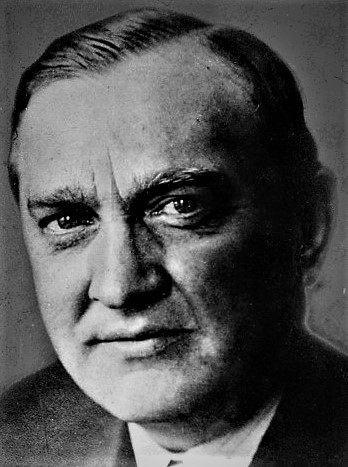
\includegraphics[width=\linewidth]{stefan-banach.jpg}\\
      {\scriptsize\color{gray}Stefan Banach (1892--1945).
      Domaine public, Wikimedia Commons.}
    \end{column}
    \begin{column}{0.72\textwidth}
      \begin{itemize}
        \item Né à Cracovie, confié à des familles d'accueil ; apprend
          une grande partie des mathématiques par lui-même.
        \item 1916 : Hugo Steinhaus surprend, dans un parc, une
          conversation de Banach sur l'intégrale de Lebesgue. Il lui
          propose des problèmes ouverts ; Banach les résout en une
          semaine. « Ma plus grande découverte scientifique a été de
          découvrir Banach. »
        \item Thèse (1920, publiée en 1922) : définit les espaces
          de Banach et fonde l'analyse fonctionnelle moderne --- le
          théorème du point fixe y apparaît.
      \end{itemize}
    \end{column}
  \end{columns}
\end{frame}

\begin{frame}{Note historique 2.3 (suite)}
  \small
  \begin{itemize}
    \item Professeur à Lwów (aujourd'hui Lviv, Ukraine), il y fonde avec
      ses collègues l'école mathématique de Lwów.
    \item On se réunit au Café Écossais ; les problèmes ouverts
      sont consignés dans un cahier resté célèbre : le Livre
      écossais.
    \item Sous l'occupation allemande, il échappe à la déportation en
      travaillant comme « nourricier de poux » dans un institut de
      recherche sur le typhus --- emploi qui protégeait alors de
      nombreux universitaires.
    \item Il meurt d'un cancer du poumon en 1945, peu après la fin de la
      guerre, à $53$ ans.
  \end{itemize}
\end{frame}

\begin{frame}{Note historique 2.4 --- Origines et applications du théorème}
  \small
  \begin{itemize}
    \item Picard (1890) utilise déjà les approximations
      successives pour l'existence et l'unicité des solutions de
      certaines équations différentielles (théorème de
      Picard-Lindelöf).
    \item Banach (1922) : le cadre abstrait. En isolant
      la complétude et le caractère contractant, un seul résultat
      couvre de nombreux problèmes.
    \item Caccioppoli (1930) le redécouvre indépendamment :
      théorème de Banach-Caccioppoli.
  \end{itemize}
  \vspace{4pt}
  Applications : construction des fractales (chapitre 3) ;
  Newton et autres méthodes numériques ; PageRank, qui a classé
  les pages web chez Google à ses débuts --- le point fixe d'une
  contraction dans un espace de dimension égale au nombre de pages du
  Web (chapitre 4).
\end{frame}

% ═══════════════════════════════════════════════════════════════════════
\section{Synthèse}
% ═══════════════════════════════════════════════════════════════════════

\begin{frame}{Ce qu'il faut retenir}
  \small
  \begin{itemize}
    \item Une métrique : quatre axiomes (positivité,
      séparation, symétrie, inégalité triangulaire) --- sur
      n'importe quel ensemble.
    \item Un même ensemble peut porter plusieurs métriques ($\dE$,
      $\dT$) ; la forme des boules en dépend.
    \item Des métriques « appliquées » : distance sphérique
      (navigation), distance de Hamming (codes correcteurs).
    \item Ouvert, fermé, compact ; dans $\R^n$,
      compact = fermé et borné (Heine-Borel).
    \item La distance de Hausdorff fait de $\Comp{E}$ un espace
      métrique dont les points sont des ensembles.
    \item Complétude : toute suite de Cauchy converge dans
      l'espace ($\R^n$ oui, $\Q$ non).
    \item Banach : dans un espace complet, une contraction a un
      unique point fixe, atteint en itérant depuis n'importe où, avec
      une erreur en $k^n/(1-k)$.
  \end{itemize}
\end{frame}

\begin{frame}{Le théorème de Banach, une dernière fois}
  \FigBox[0.36\textheight]{%
    \begin{tikzpicture}[
        hyp/.style={draw=sectioncolor, fill=thmboxbg, rounded corners=2pt,
          thick, align=center, font=\small, minimum height=1.1cm,
          text width=3.2cm},
        conc/.style={hyp, draw=coveraccent!85!black, fill=secboxbg,
          text width=4.4cm}]
      \node[hyp] (e) at (0,0.75) {$(E,d)$ complet};
      \node[hyp] (f) at (0,-0.75) {$f$ contraction\\$k<1$};
      \node[conc] (c) at (6.2,0) {un unique $\overline{x}$\\
        $f^n(x_0)\to\overline{x}$ pour tout $x_0$\\
        erreur $\leq\frac{k^n}{1-k}\,d(x_0,x_1)$};
      \draw[fleche] (e.east) -- (c.west);
      \draw[fleche] (f.east) -- (c.west);
    \end{tikzpicture}}
  \small
  \begin{center}
  \begin{tabular}{ll}
    \toprule
    Espace complet & Ce qu'on y trouve comme point fixe \\
    \midrule
    $I\subset\R$ fermé & le zéro cherché par la méthode de Newton \\
    $\big(\Comp{\R^2},\dH\big)$ & une fractale (chapitre 3) \\
    vecteurs de probabilité & le classement PageRank (chapitre 4) \\
    \bottomrule
  \end{tabular}
  \end{center}
\end{frame}


\end{document}
